% !TeX program = xelatex
\documentclass[UTF8]{ctexart}
\usepackage[margin=1in]{geometry}
\usepackage{graphicx}
\usepackage{caption}
\usepackage{hyperref}

\graphicspath{{../images/}{../chunks/images/}{images/}}
\setlength{\parindent}{0pt}
\setlength{\parskip}{0.6em}

\newenvironment{english}{\par\small\noindent\textbf{原文}\quad\ignorespaces}{\par}
\newenvironment{zhtranslation}{\par\noindent\textbf{译文}\quad\ignorespaces}{\par\vspace{0.35em}}

\begin{document}

\part*{Henri Poincaré, \emph{Science and Method}\\亨利·庞加莱《科学与方法》}

\section*{I. The Selection of Facts\\一、事实的选择}

\begin{english}
Tolstoi explains somewhere in his writings why, in his opinion, “Science for Science's sake” is an absurd conception. We cannot know all the facts, since they are practically infinite in number. We must make a selection; and that being so, can this selection be governed by the mere caprice of our curiosity? Is it not better to be guided by utility, by our practical, and more especially our moral, necessities? Have we not some better occupation than counting the number of ladybirds in existence on this planet?
\end{english}
\begin{zhtranslation}
托尔斯泰在某处著作中解释过，为什么在他看来，“为科学而科学”是一种荒谬的观念。我们不可能认识所有事实，因为事实的数量实际上是无限的。我们必须作出选择；既然如此，这种选择能只由好奇心的一时任性来支配吗？由功用，由我们的实践需要，尤其由我们的道德需要来引导，不是更好吗？难道我们没有比清点地球上有多少只瓢虫更值得做的事吗？\end{zhtranslation}

\begin{english}
It is clear that for him the word utility has not the meaning assigned to it by business men, and, after them, by the greater number of our contemporaries. He cares but little for the industrial applications of science, for the marvels of electricity or of automobilism, which he regards rather as hindrances to moral progress. For him the useful is exclusively what is capable of making men better.
\end{english}
\begin{zhtranslation}
显然，对他来说，“功用”一词并不是商人以及随后多数当代人赋予它的含义。他几乎不关心科学的工业应用，不关心电力或汽车技术的奇迹；在他看来，这些倒更像是道德进步的障碍。对他而言，有用的东西只限于能够使人变得更好的东西。\end{zhtranslation}

\begin{english}
It is hardly necessary for me to state that, for my part, I could not be satisfied with either of these ideals. I have no liking either for a greedy and narrow plutocracy, or for a virtuous unaspiring democracy, solely occupied in turning the other cheek, in which we should find good people devoid of curiosity, who, avoiding all excesses, would not die of any disease--save boredom. But it is all a matter of taste, and that is not the point I wish to discuss.
\end{english}
\begin{zhtranslation}
几乎无须说明，就我而言，我不能满足于这两种理想中的任何一种。我既不喜欢贪婪而狭隘的富豪政治，也不喜欢一种有德却无所追求的民主社会，在那里，人们只忙着“把另一边脸也转过去”；那里有善良却没有好奇心的人，他们避开一切过度，除了无聊之外不会死于任何疾病。不过这全是趣味问题，并不是我想讨论的要点。\end{zhtranslation}

\begin{english}
Nonetheless the question remains, and it claims our attention. If our selection is only determined by caprice or by immediate necessity, there can be no science for science's sake, and consequently no science. Is this true? There is no disputing the fact that a selection must be made: however great our activity, facts outstrip us, and we can never overtake them; while the scientist is discovering one fact, millions and millions are produced in every cubic inch of his body. Trying to make science contain nature is like trying to make the part contain the whole.
\end{english}
\begin{zhtranslation}
然而问题依然存在，而且需要我们认真对待。如果我们的选择只由任性或眼前需要决定，那么就不会有“为科学而科学”，因而也不会有科学。事实真是如此吗？选择必须作出，这是无可争辩的：无论我们多么勤奋，事实总是跑在我们前面，我们永远追不上它们；科学家发现一个事实的同时，他身体每一立方英寸里又产生了成千上万的事实。想让科学容纳自然，就像想让部分容纳整体。\end{zhtranslation}

\begin{english}
But scientists believe that there is a hierarchy of facts, and that a judicious selection can be made. They are right, for otherwise there would be no science, and science does exist. One has only to open one's eyes to see that the triumphs of industry, which have enriched so many practical men, would never have seen the light if only these practical men had existed, and if they had not been preceded by disinterested fools who died poor, who never thought of the useful, and yet had a guide that was not their own caprice.
\end{english}
\begin{zhtranslation}
但是科学家相信，事实之间有一种层级，并且可以作出明智的选择。他们是对的；否则科学就不会存在，而科学确实存在。只要睁开眼睛就能看见，那些使许多实际人物致富的工业胜利，如果世界上只有这些实际人物，如果在他们之前没有那些无私的傻子，便绝不会出现。这些人穷困而死，从未想着“有用”，但他们仍有某种指引，而那并不是他们自己的任性。\end{zhtranslation}

\begin{english}
What these fools did, as Mach has said, was to save their successors the trouble of thinking. If they had worked solely in view of an immediate application, they would have left nothing behind them, and in face of a new requirement, all would have had to be done again. Now the majority of men do not like thinking, and this is perhaps a good thing, since instinct guides them, and very often better than reason would guide a pure intelligence, at least whenever they are pursuing an end that is immediate and always the same. But instinct is routine, and if it were not fertilized by thought, it would advance no further with man than with the bee or the ant. It is necessary, therefore, to think for those who do not like thinking, and as they are many, each one of our thoughts must be useful in as many circumstances as possible. For this reason, the more general a law is, the greater is its value.
\end{english}
\begin{zhtranslation}
正如马赫所说，这些傻子所做的，是替后来者省去了思考的麻烦。如果他们只为了眼前的应用而工作，他们就不会留下任何东西；一旦出现新的需求，一切都得从头再来。多数人并不喜欢思考，这也许还是好事，因为本能会引导他们；至少当他们追求的是眼前而且总是相同的目标时，本能常常比纯粹理智更能引导他们。但是本能只是惯例；如果没有思想使它受孕，它在人那里也不会比在蜜蜂或蚂蚁那里走得更远。因此，必须为那些不喜欢思考的人思考；而这样的人很多，所以我们的每一个思想都应当在尽可能多的情形中有用。正因为如此，一条定律越普遍，它的价值就越大。\end{zhtranslation}

\begin{english}
This shows us how our selection should be made. The most interesting facts are those which can be used several times, those which have a chance of recurring. We have been fortunate enough to be born in a world where there are such facts. Suppose that instead of eighty chemical elements we had eighty million, and that they were not some common and others rare, but uniformly distributed. Then each time we picked up a new pebble there would be a strong probability that it was composed of some unknown substance. Nothing that we knew of other pebbles would tell us anything about it. Before each new object we should be like a newborn child; like him we could but obey our caprices or our necessities. In such a world there would be no science; perhaps thought and even life would be impossible, since evolution could not have developed the instincts of self-preservation. Providentially it is not so; but this blessing, like all those to which we are accustomed, is not appreciated at its true value. The biologist would be equally embarrassed if there were only individuals and no species, and if heredity did not make children resemble their parents.
\end{english}
\begin{zhtranslation}
这就向我们说明，应当怎样作出选择。最有意思的事实，是那些能够被多次使用的事实，是那些有可能重复出现的事实。我们足够幸运，出生在一个确有这类事实的世界里。设想一下，如果化学元素不是八十种，而是八千万种；而且它们并非有的常见、有的稀少，而是均匀分布。那么我们每捡起一块新的卵石，它很可能都由某种未知物质组成。我们关于其他卵石所知道的一切，都不会告诉我们关于它的任何事情。面对每一个新对象，我们都会像新生儿一样；像他一样，我们只能听从自己的任性或需要。在这样的世界里就不会有科学；也许思想甚至生命都不可能存在，因为进化无法发展出自我保存的本能。幸而事实并非如此；但这种恩惠也和一切我们习以为常的恩惠一样，并没有得到应有的珍视。如果只有个体而没有物种，如果遗传不能使子女与父母相似，生物学家也会同样无所适从。\end{zhtranslation}

\begin{english}
Which, then, are the facts that have a chance of recurring? In the first place, simple facts. It is evident that in a complex fact many circumstances are united by chance, and that only a still more improbable chance could ever so unite them again. But are there such things as simple facts? and if there are, how are we to recognize them? Who can tell that what we believe to be simple does not conceal an alarming complexity? All that we can say is that we must prefer facts which appear simple, to those in which our rude vision detects dissimilar elements. Then only two alternatives are possible; either this simplicity is real, or else the elements are so intimately mingled that they do not admit of being distinguished. In the first case we have a chance of meeting the same simple fact again, either in all its purity, or itself entering as an element into some complex whole. In the second case the intimate mixture has similarly a greater chance of being reproduced than a heterogeneous assemblage. Chance can mingle, but it cannot unmingle, and a combination of various elements in a well-ordered edifice in which something can be distinguished, can only be made deliberately. There is, therefore, but little chance that an assemblage in which different things can be distinguished should ever be reproduced. On the other hand, there is great probability that a mixture which appears homogeneous at first sight will be reproduced several times. Accordingly facts which appear simple, even if they are not so in reality, will be more easily brought about again by chance.
\end{english}
\begin{zhtranslation}
那么，哪些事实有可能重复出现呢？首先是简单事实。显然，在一个复杂事实中，许多情形是由偶然性结合在一起的；只有一种更不可能的偶然性，才会再次以同样方式把它们结合起来。但是，真有简单事实这种东西吗？如果有，我们又如何识别它们？谁能断言，我们以为简单的东西没有隐藏着惊人的复杂性？我们所能说的只是：我们必须偏爱那些看起来简单的事实，而不是那些在我们粗糙的眼光中显出异质成分的事实。于是只有两种可能：这种简单性是真实的；或者，各个成分混合得如此紧密，以致无法加以区分。在第一种情形中，我们有机会再次遇到同一个简单事实，或者以其纯粹形态出现，或者作为一个成分进入某个复杂整体。在第二种情形中，这种紧密混合也比异质拼合更有可能重现。偶然性能混合，却不能解混；由多种元素构成、秩序井然而且其中某些东西可被区分的组合，只能有意造成。因此，一个其中可以区分出不同事物的集合几乎没有机会被再次重现。相反，一个乍看之下同质的混合物，多次重现的概率却很大。所以，那些看起来简单的事实，即使实际上并不简单，也更容易被偶然性再次带来。\end{zhtranslation}

\begin{english}
It is this that justifies the method instinctively adopted by scientists, and what perhaps justifies it still better is that facts which occur frequently appear to us simple just because we are accustomed to them.
\end{english}
\begin{zhtranslation}
正是这一点为科学家本能采用的方法提供了根据；也许更能为它辩护的是，频繁发生的事实之所以在我们看来简单，正是因为我们已经习惯了它们。\end{zhtranslation}

\begin{english}
But where is the simple fact? Scientists have tried to find it in the two extremes, in the infinitely great and in the infinitely small. The astronomer has found it because the distances of the stars are immense, so great that each of them appears only as a point and qualitative differences disappear, and because a point is simpler than a body which has shape and qualities. The physicist, on the other hand, has sought the elementary phenomenon in an imaginary division of bodies into infinitely small atoms, because the conditions of the problem, which undergo slow and continuous variations as we pass from one point of the body to another, may be regarded as constant within each of these little atoms. Similarly the biologist has been led instinctively to regard the cell as more interesting than the whole animal, and the event has proved him right, since cells belonging to the most diverse organisms have greater resemblances, for those who can recognize them, than the organisms themselves. The sociologist is in a more embarrassing position. The elements, which for him are men, are too dissimilar, too variable, too capricious, in a word, too complex themselves. Furthermore, history does not repeat itself; how, then, is he to select the interesting fact, the fact which is repeated? Method is precisely the selection of facts, and accordingly our first care must be to devise a method. Many have been devised because none holds the field undisputed. Nearly every sociological thesis proposes a new method, which, however, its author is very careful not to apply, so that sociology is the science with the greatest number of methods and the least results.
\end{english}
\begin{zhtranslation}
但是，简单事实在哪里呢？科学家曾试图在两个极端中寻找它：在无限大和无限小之中。天文学家找到了它，因为恒星之间的距离极其巨大，大到每一颗星看起来都只是一个点，性质上的差别消失了；而一个点比有形状、有性质的物体更简单。另一方面，物理学家则在把物体设想为无限小原子的划分中寻找基本现象，因为问题的条件在我们从物体一点移到另一点时缓慢而连续地变化，在每一个这样的小原子内部却可以被看作恒定。同样，生物学家也本能地被引导，把细胞看得比整个动物更有意思；结果证明他是对的，因为在能够识别这些相似性的人看来，属于最不同有机体的细胞之间，比这些有机体本身之间有更多相似之处。社会学家的处境则更尴尬。对他来说，组成元素是人；而人太不相同，太多变，太任性，简言之，本身就太复杂。此外，历史不会重复；那么，他怎样选择有意思的事实，怎样选择会重复的事实呢？方法恰恰就是事实的选择；因此我们的首要任务就是设计一种方法。人们已经设计出许多方法，因为没有一种能毫无争议地占据主导。几乎每一篇社会学论文都会提出一种新方法，不过作者总是十分谨慎地不去运用它；于是社会学便成了方法最多、成果最少的科学。\end{zhtranslation}

\begin{english}
It is with regular facts, therefore, that we ought to begin; but as soon as the rule is well established, as soon as it is no longer in doubt, the facts which are in complete conformity with it lose their interest, since they can teach us nothing new. Then it is the exception which becomes important. We cease to look for resemblances, and apply ourselves before all else to differences, and of these differences we select first those that are most accentuated, not only because they are the most striking, but because they will be the most instructive. This will be best explained by a simple example. Suppose we are seeking to determine a curve by observing some of the points on it. The practical man who looked only to immediate utility would merely observe the points he required for some special object; these points would be badly distributed on the curve, they would be crowded together in certain parts and scarce in others, so that it would be impossible to connect them by a continuous line, and they would be useless for any other application. The scientist would proceed in a different manner. Since he wishes to study the curve for itself, he will distribute the points to be observed regularly, and as soon as he knows some of them, he will join them by a regular line, and he will then have the complete curve. But how is he to accomplish this? If he has determined one extreme point on the curve, he will not remain close to this extremity, but will move to the other end. After the two extremities, the central point is the most instructive, and so on.
\end{english}
\begin{zhtranslation}
因此，我们应当从有规律的事实开始；但是，一旦规则已经确立，一旦它不再可疑，与它完全符合的事实就失去了兴趣，因为它们不能教给我们任何新东西。于是例外变得重要。我们不再寻找相似，而首先致力于差异；在这些差异中，我们又首先选择最显著的差异，不仅因为它们最醒目，还因为它们最有教益。一个简单例子最能说明这一点。假定我们要通过观察曲线上的若干点来确定一条曲线。只看眼前功用的实际人物，只会观察为某个特殊目的所需的点；这些点在曲线上分布很差，有的部分挤在一起，有的部分稀疏，以致无法把它们连成一条连续曲线，而且对任何其他应用都毫无用处。科学家的做法不同。既然他想研究曲线本身，他就会有规则地分布要观察的点；一旦知道其中一些点，他就会用一条有规则的线把它们连接起来，从而得到完整曲线。但他怎样做到这一点呢？如果他已经确定曲线的一个端点，他不会停留在这个端点附近，而会移向另一端。在两个端点之后，最有教益的是中心点，如此继续下去。\end{zhtranslation}

\begin{english}
Thus when a rule has been established, we have first to look for the cases in which the rule stands the best chance of being found in fault. This is one of many reasons for the interest of astronomical facts and of geological ages. By making long excursions in space or in time, we may find our ordinary rules completely upset, and these great upsettings will give us a clearer view and better comprehension of such small changes as may occur nearer us, in the small corner of the world in which we are called to live and move. We shall know this corner better for the journey we have taken into distant lands where we had no concern.
\end{english}
\begin{zhtranslation}
因此，当一条规则已经确立时，我们首先要寻找那些最可能让这条规则出错的情形。这是天文学事实和地质年代之所以令人感兴趣的许多理由之一。通过在空间或时间中作长距离远行，我们也许会发现我们的通常规则被完全颠覆；这些巨大的颠覆会使我们更清楚地看见、更好地理解那些可能发生在我们近旁的小变化，发生在我们被召唤来生活和活动的世界小角落里的变化。正因为我们曾经到那些与我们无关的远方去旅行，我们会更好地认识这个角落。\end{zhtranslation}

\begin{english}
But what we must aim at is not so much to ascertain resemblances and differences, as to discover similarities hidden under apparent discrepancies. The individual rules appear at first discordant, but on looking closer we can generally detect a resemblance; though differing in matter, they approximate in form and in the order of their parts. When we examine them from this point of view, we shall see them widen and tend to embrace everything. This is what gives a value to certain facts that come to complete a whole, and show that it is the faithful image of other known wholes.
\end{english}
\begin{zhtranslation}
不过，我们的目标与其说是确认相似和差异，不如说是发现隐藏在表面分歧之下的相似性。各个规则起初看起来并不协调，但细看之下，我们通常能够发现一种相似；它们在材料上不同，却在形式以及各部分的秩序上相近。当我们从这个角度考察它们时，就会看到它们扩展并趋向于包容一切。某些事实之所以有价值，正是因为它们来补全一个整体，并显示这个整体是其他已知整体的忠实映像。\end{zhtranslation}

\begin{english}
I cannot dwell further on this point, but these few words will suffice to show that the scientist does not make a random selection of the facts to be observed. He does not count ladybirds, as Tolstoi says, because the number of these insects, interesting as they are, is subject to capricious variations. He tries to condense a great deal of experience and a great deal of thought into a small volume, and that is why a little book on physics contains so many past experiments, and a thousand times as many possible ones, whose results are known in advance.
\end{english}
\begin{zhtranslation}
我不能在这一点上继续展开，但这几句话足以说明，科学家并不是随意选择要观察的事实。他并不像托尔斯泰所说的那样去数瓢虫，因为这些昆虫固然有趣，其数量却受任意变化支配。他试图把大量经验和大量思想压缩进一个小体积之中；正因为如此，一本小小的物理学书里包含了那么多过去的实验，也包含了多出千倍的可能实验，而这些实验的结果已经可以预先知道。\end{zhtranslation}

\begin{english}
But so far we have only considered one side of the question. The scientist does not study nature because it is useful to do so. He studies it because he takes pleasure in it, and he takes pleasure in it because it is beautiful. If nature were not beautiful it would not be worth knowing, and life would not be worth living. I am not speaking, of course, of that beauty which strikes the senses, of the beauty of qualities and appearances. I am far from despising this, but it has nothing to do with science. What I mean is that more intimate beauty which comes from the harmonious order of its parts, and which a pure intelligence can grasp. It is this that gives a body, so to speak, a skeleton to the shimmering visions that flatter our senses, and without this support the beauty of these fleeting dreams would be imperfect, because it would be indefinite and ever elusive. Intellectual beauty, on the contrary, is self-sufficing, and it is for it, more perhaps than for the future good of humanity, that the scientist condemns himself to long and painful labours.
\end{english}
\begin{zhtranslation}
但是到目前为止，我们只考察了问题的一面。科学家研究自然，并不是因为这样做有用。他研究自然，是因为他从中得到乐趣；而他从中得到乐趣，是因为自然是美的。如果自然不美，它就不值得被认识，生活也不值得过下去。当然，我说的并不是打动感官的那种美，不是性质和外观的美。我绝不轻视这种美，但它与科学无关。我所说的是一种更内在的美，它来自各部分和谐的秩序，纯粹理智能够把握它。可以说，正是这种美给那些取悦我们感官的闪烁幻象赋予了骨架；没有这种支撑，这些转瞬即逝的梦幻之美就是不完善的，因为它会是不确定的、永远逃逸的。相反，理智之美自足自立；科学家甘愿承受漫长而痛苦的劳动，也许更多是为了它，而不是为了人类未来的利益。\end{zhtranslation}

\begin{english}
It is, then, the search for this special beauty, the sense of the harmony of the world, that makes us select the facts best suited to contribute to this harmony; just as the artist selects those features of his sitter which complete the portrait and give it character and life. And there is no fear that this instinctive and unacknowledged preoccupation will divert the scientist from the search for truth. We may dream of a harmonious world, but how far it will fall short of the real world! The Greeks, the greatest artists that ever were, constructed a heaven for themselves; how poor a thing it is beside the heaven as we know it!
\end{english}
\begin{zhtranslation}
因此，正是对这种特殊美的追求，正是对世界和谐的感受，使我们选择那些最适合促成这种和谐的事实；这就像艺术家会选择模特身上那些能完成肖像、赋予肖像性格和生命的特征一样。无需担心这种本能的、未被承认的关切会使科学家偏离对真理的追求。我们也许会梦想一个和谐的世界，但它离真实世界会相差多远！希腊人是有史以来最伟大的艺术家，他们为自己建构了一个天空；与我们今日所知的天空相比，那是何等贫乏！
\end{zhtranslation}

\begin{english}
It is because simplicity and vastness are both beautiful that we seek by preference simple facts and vast facts; that we take delight, now in following the giant courses of the stars, now in scrutinizing with a microscope that prodigious smallness which is also a vastness, and now in seeking in geological ages the traces of a past that attracts us because of its remoteness.
\end{english}
\begin{zhtranslation}
正因为简单性和广大性都是美的，我们才优先寻找简单事实和宏大事实；我们时而乐于追随群星巨大的轨道，时而乐于用显微镜审视那同样也是一种广大的惊人微小，时而又在地质年代中寻找遥远过去的痕迹，而正是这种遥远吸引着我们。\end{zhtranslation}

\begin{english}
Thus we see that care for the beautiful leads us to the same selection as care for the useful. Similarly economy of thought, that economy of effort which, according to Mach, is the constant tendency of science, is a source of beauty as well as a practical advantage. The buildings we admire are those in which the architect has succeeded in proportioning the means to the end, in which the columns seem to carry the burdens imposed on them lightly and without effort, like the graceful caryatids of the Erechtheum.
\end{english}
\begin{zhtranslation}
由此可见，对美的关切会把我们引向与对有用性的关切相同的选择。同样，思想的经济性，即马赫所说的科学恒常倾向于追求的努力经济性，既是实践上的优点，也是美的源泉。我们所赞赏的建筑，是建筑师成功地使手段与目的相称的建筑；在那里，柱子似乎轻盈而毫不费力地承受着加在它们身上的负荷，就像厄瑞克忒翁神庙中优雅的女像柱。\end{zhtranslation}

\begin{english}
Whence comes this concordance? Is it merely that things which seem to us beautiful are those which are best adapted to our intelligence, and that consequently they are at the same time the tools that intelligence knows best how to handle? Or is it due rather to evolution and natural selection? Have the peoples whose ideal conformed best to their own interests, properly understood, exterminated the others and taken their place? One and all pursued their ideal without considering the consequences, but while this pursuit led some to their destruction, it gave empire to others. We are tempted to believe this, for if the Greeks triumphed over the barbarians, and if Europe, heir of the thought of the Greeks, dominates the world, it is due to the fact that the savages loved garish colours and the blatant noise of the drum, which appealed to their senses, while the Greeks loved the intellectual beauty hidden behind sensible beauty, and that it is this beauty which gives certainty and strength to the intelligence.
\end{english}
\begin{zhtranslation}
这种一致从何而来？是否只是因为那些在我们看来美的东西，正是最适合我们理智的东西，因而同时也是理智最懂得如何运用的工具？或者，它更应归因于进化和自然选择？那些理想最符合自身真正利益的民族，是否消灭了其他民族并取而代之？所有民族都追求自己的理想，并不考虑后果；但这种追求有的把人引向毁灭，有的却赋予人以统治力。我们很容易相信这一点，因为如果希腊人战胜了蛮族，如果继承希腊思想的欧洲支配了世界，那是因为野蛮人喜爱刺眼的色彩和喧嚣的鼓声，这些诉诸感官；而希腊人热爱隐藏在感性美之后的理智之美，正是这种美给予理智以确定性和力量。\end{zhtranslation}

\begin{english}
No doubt Tolstoi would be horrified at such a triumph, and he would refuse to admit that it could be truly useful. But this disinterested pursuit of truth for its own beauty is also wholesome, and can make men better. I know very well there are disappointments, that the thinker does not always find the serenity he should, and even that some scientists have thoroughly bad tempers.
\end{english}
\begin{zhtranslation}
托尔斯泰无疑会对这样的胜利感到震惊，并拒绝承认它可能真正有用。但是，这种为了真理自身之美而无私追求真理的活动，也同样有益健康，并能使人变得更好。我当然知道，其中会有失望；思想者并不总能获得他本应拥有的宁静，甚至有些科学家的脾气还糟糕透顶。\end{zhtranslation}

\begin{english}
Must we therefore say that science should be abandoned, and morality alone be studied? Does anyone suppose that moralists themselves are entirely above reproach when they have come down from the pulpit?
\end{english}
\begin{zhtranslation}
因此我们就必须说应当放弃科学，只研究道德吗？难道有人以为，道德家一旦从讲坛上走下来，他们自己就完全无可指摘吗？
\end{zhtranslation}

\begin{center}
[\dots]
\end{center}

\section*{III. Mathematical Discovery\\三、数学发现}

\begin{english}
The genesis of mathematical discovery is a problem which must inspire the psychologist with the keenest interest. For this is the process in which the human mind seems to borrow least from the exterior world, in which it acts, or appears to act, only by itself and on itself, so that by studying the process of geometric thought we may hope to arrive at what is most essential in the human mind.
\end{english}
\begin{zhtranslation}
数学发现的发生，是一个必定会引起心理学家最强烈兴趣的问题。因为在这一过程中，人类心智似乎最少向外部世界借取东西；它只凭自身并作用于自身，或者看起来如此。因此，通过研究几何思想的过程，我们也许有希望抵达人类心智中最本质的东西。\end{zhtranslation}

\begin{english}
This has long been understood, and a few months ago a review called \emph{L'Enseignement mathématique}, edited by MM. Laisant and Fehr, instituted an enquiry into the habits of mind and methods of work of different mathematicians. I had outlined the principal features of this article when the results of the enquiry were published, so that I have hardly been able to make any use of them, and I will content myself with saying that the majority of the evidence confirms my conclusions. I do not say there is unanimity, for on an appeal to universal suffrage we cannot hope to obtain unanimity.
\end{english}
\begin{zhtranslation}
这一点早已为人所理解。几个月前，由莱桑和费尔二位先生编辑的《数学教育》杂志，发起了一项调查，研究不同数学家的思维习惯和工作方法。当调查结果发表时，本文的主要轮廓我已经拟好，所以几乎没有能够利用这些材料；我只满足于说，大多数证据都证实了我的结论。我并不说意见完全一致，因为诉诸普遍投票时，我们不能指望得到全体一致。\end{zhtranslation}

\begin{english}
One first fact must astonish us, or rather would astonish us if we were not too much accustomed to it. How does it happen that there are people who do not understand mathematics? If the science invokes only the rules of logic, those accepted by all well-formed minds, if its evidence is founded on principles that are common to all men, and that none but a madman would attempt to deny, how does it happen that there are so many people who are entirely impervious to it?
\end{english}
\begin{zhtranslation}
首先有一个事实必定使我们惊讶，或者说，如果我们不是已经太习惯于它，它本来会使我们惊讶：为什么会有人不理解数学？如果这门科学所诉诸的只是逻辑规则，只是所有健全心智都承认的规则；如果它的证据建立在所有人共有、除了疯子无人会试图否认的原则之上，那么为什么竟有那么多人对它完全不能领会？
\end{zhtranslation}

\begin{english}
There is nothing mysterious in the fact that everyone is not capable of discovery. That everyone should not be able to retain a demonstration he has once learnt is still comprehensible. But what does seem most surprising, when we consider it, is that anyone should be unable to understand a mathematical argument at the very moment it is stated to him. And yet those who can only follow the argument with difficulty are in a majority; this is incontestable, and the experience of teachers of secondary education will certainly not contradict me.
\end{english}
\begin{zhtranslation}
并非每个人都能作出发现，这并不神秘。一个人学过一个证明之后不能把它记住，这仍然可以理解。但是认真想来，最令人惊讶的似乎是：有人竟然在一个数学论证正向他陈述的当下就不能理解它。然而，只有困难地跟上论证的人占多数；这一点无可争辩，中学教师的经验当然也不会反驳我。\end{zhtranslation}

\begin{english}
And still further, how is error possible in mathematics? A healthy intellect should not be guilty of any error in logic, and yet there are very keen minds which will not make a false step in a short argument such as those we have to make in the ordinary actions of life, which yet are incapable of following or repeating without error the demonstrations of mathematics which are longer, but which are, after all, only accumulations of short arguments exactly analogous to those they make so easily. Is it necessary to add that mathematicians themselves are not infallible?
\end{english}
\begin{zhtranslation}
再进一步说，数学中的错误怎么可能发生？一个健全的理智不应当犯任何逻辑错误；然而，有些非常敏锐的头脑，在日常生活行动中所需的短论证里不会走错一步，却无法无误地跟随或复述较长的数学证明，尽管这些证明归根到底只是许多短论证的累积，而这些短论证恰好与他们轻易作出的那些完全类似。还需要补充说，数学家本人也并非不会犯错吗？\end{zhtranslation}

\begin{english}
The answer appears to me obvious. Imagine a long series of syllogisms in which the conclusions of those that precede form the premises of those that follow. We shall be capable of grasping each of the syllogisms, and it is not in the passage from premises to conclusion that we are in danger of going astray. But between the moment when we meet a proposition for the first time as the conclusion of one syllogism, and the moment when we find it once more as the premise of another syllogism, much time will sometimes have elapsed, and we shall have unfolded many links of the chain; accordingly it may well happen that we shall have forgotten it, or, what is more serious, forgotten its meaning. So we may chance to replace it by a somewhat different proposition, or to preserve the same statement but give it a slightly different meaning, and thus we are in danger of falling into error.
\end{english}
\begin{zhtranslation}
在我看来，答案是显而易见的。设想一长串三段论，前面三段论的结论构成后面三段论的前提。我们能够把握每一个三段论；危险并不在于从前提过渡到结论的那一步。但是，从我们第一次把某个命题作为一个三段论的结论遇到它，到我们再次把它作为另一个三段论的前提发现它，这中间有时会经过很长时间，我们也已经展开了链条中的许多环节。因此，很可能发生的情况是，我们已经忘记了它，或者更严重地说，忘记了它的意义。于是我们可能偶然用一个略有不同的命题替代它，或者保留同一个表述，却赋予它稍稍不同的意义；这样我们就有陷入错误的危险。\end{zhtranslation}

\begin{english}
A mathematician must often use a rule, and, naturally, he begins by demonstrating the rule. At the moment the demonstration is quite fresh in his memory he understands perfectly its meaning and significance, and he is in no danger of changing it. But later on he commits it to memory, and only applies it in a mechanical way, and then, if his memory fails him, he may apply it wrongly. It is thus, to take a simple and almost vulgar example, that we sometimes make mistakes in calculation, because we have forgotten our multiplication table.
\end{english}
\begin{zhtranslation}
数学家常常必须使用一条规则；自然，他一开始会证明这条规则。当证明在记忆中还十分新鲜时，他完全理解它的含义和意义，也没有改变它的危险。但后来他把它交给记忆，只是以机械方式加以应用；这时如果记忆失灵，他就可能用错。举一个简单得几乎粗俗的例子，我们有时会在计算中出错，正是因为忘记了乘法表。\end{zhtranslation}

\begin{english}
On this view special aptitude for mathematics would be due to nothing but a very certain memory or a tremendous power of attention. It would be a quality analogous to that of the whist player who can remember the cards played, or, to rise a step higher, to that of the chess player who can picture a very great number of combinations and retain them in his memory. Every good mathematician should also be a good chess player and vice versa, and similarly he should be a good numerical calculator. Certainly this sometimes happens, and thus Gauss was at once a geometrician of genius and a very precocious and very certain calculator.
\end{english}
\begin{zhtranslation}
按这种看法，数学的特殊才能只不过来自非常可靠的记忆力或巨大的注意力。它会类似于惠斯特牌手能记住已经打出的牌，或者再高一步，类似于棋手能够想象大量组合并把它们保存在记忆中。每个优秀数学家也都应当是优秀棋手，反之亦然；同样，他也应当是优秀的数字计算者。当然，这种情况有时确实发生；高斯既是天才几何学家，也是一位早熟而极其可靠的计算者。\end{zhtranslation}

\begin{english}
But there are exceptions, or rather I am wrong, for I cannot call them exceptions, otherwise the exceptions would be more numerous than the cases of conformity with the rule. On the contrary, it was Gauss who was an exception. As for myself, I must confess I am absolutely incapable of doing an addition sum without a mistake. Similarly I should be a very bad chess player. I could easily calculate that by playing in a certain way I should be exposed to such and such a danger; I should then review many other moves, which I should reject for other reasons, and I should end by making the move I first examined, having forgotten in the interval the danger I had foreseen.
\end{english}
\begin{zhtranslation}
但也有例外；或者更确切地说，我说错了，因为我不能把它们称为例外，否则例外会比符合规则的情形更多。相反，高斯才是例外。至于我自己，必须承认，我完全不能保证做一个加法题而不出错。同样，我也会是一个很糟糕的棋手。我可以轻易算出，以某种方式走棋会使我暴露于某种危险；随后我会考察许多其他走法，又因别的理由把它们否定；最后我会走最初考察的那一步，却已经在这中间忘记了我曾预见的危险。\end{zhtranslation}

\begin{english}
In a word, my memory is not bad, but it would be insufficient to make me a good chess player. Why, then, does it not fail me in a difficult mathematical argument in which the majority of chess players would be lost? Clearly because it is guided by the general trend of the argument. A mathematical demonstration is not a simple juxtaposition of syllogisms; it consists of syllogisms placed in a certain order, and the order in which these elements are placed is much more important than the elements themselves. If I have the feeling, so to speak the intuition, of this order, so that I can perceive the whole of the argument at a glance, I need no longer be afraid of forgetting one of the elements; each of them will place itself naturally in the position prepared for it, without my having to make any effort of memory.
\end{english}
\begin{zhtranslation}
总之，我的记忆并不差，但它不足以使我成为一个好棋手。那么，为什么在一个困难的数学论证中，在大多数棋手都会迷失的地方，它却没有辜负我呢？显然，是因为它受到论证总体趋向的引导。数学证明并不是三段论的简单并列；它由按某种秩序安置的三段论构成，而这些元素被安置的秩序比元素本身重要得多。如果我对这种秩序有一种感觉，或者说一种直觉，以至于能够一眼看见论证的整体，我就不必再害怕忘记其中某个元素；每个元素都会自然地安放到为它准备的位置上，而无需我作任何记忆努力。\end{zhtranslation}

\begin{english}
It seems to me, then, as I repeat an argument I have learnt, that I could have discovered it. This is often only an illusion; but even then, even if I am not clever enough to create for myself, I rediscover it myself as I repeat it.
\end{english}
\begin{zhtranslation}
因此，当我复述一个已经学过的论证时，我似乎觉得自己本来也能够发现它。这常常只是一种幻觉；但即便如此，即便我并不聪明到能够自行创造，我在复述它时也仍是在亲自重新发现它。\end{zhtranslation}

\begin{english}
We can understand that this feeling, this intuition of mathematical order, which enables us to guess hidden harmonies and relations, cannot belong to everyone. Some have neither this delicate feeling that is difficult to define, nor a power of memory and attention above the common, and so they are absolutely incapable of understanding even the first steps of higher mathematics. This applies to the majority of people. Others have the feeling only in a slight degree, but they are gifted with an uncommon memory and a great capacity for attention. They learn the details one after the other by heart, they can understand mathematics and sometimes apply them, but they are not in a condition to create. Lastly, others possess the special intuition I have spoken of more or less highly developed, and they cannot only understand mathematics, even though their memory is in no way extraordinary, but they can become creators, and seek to make discovery with more or less chance of success, according as their intuition is more or less developed.
\end{english}
\begin{zhtranslation}
我们可以理解，这种感觉，这种对数学秩序的直觉，使我们能够猜出隐藏的和谐与关系，但它不可能属于每一个人。有些人既没有这种难以界定的微妙感觉，也没有超出常人的记忆力和注意力，所以他们甚至完全无法理解高等数学的最初几步。多数人就是如此。另一些人只在很轻微的程度上具有这种感觉，却拥有非同寻常的记忆力和很强的注意力。他们把细节一个接一个地背下来，能够理解数学，有时也能应用数学，但他们并不具备创造的条件。最后，还有一些人或多或少高度发展了我所说的特殊直觉；即便他们的记忆并无任何非凡之处，他们不仅能理解数学，而且能够成为创造者，并依其直觉发展程度的高低，在或大或小的成功机会中寻求发现。\end{zhtranslation}

\begin{english}
What, in fact, is mathematical discovery? It does not consist in making new combinations with mathematical entities that are already known. That can be done by anyone, and the combinations that could be so formed would be infinite in number, and the greater part of them would be absolutely devoid of interest. Discovery consists precisely in not constructing useless combinations, but in constructing those that are useful, which are an infinitely small minority. Discovery is discernment, selection.
\end{english}
\begin{zhtranslation}
那么，数学发现究竟是什么？它并不在于用已经知道的数学对象作出新的组合。任何人都能这样做，而能够这样形成的组合数量是无限的，其中绝大部分毫无兴趣。发现恰恰在于不构造无用组合，而构造那些有用的组合；后者只是无限小的少数。发现就是辨别，就是选择。\end{zhtranslation}

\begin{english}
How this selection is to be made I have explained above. Mathematical facts worthy of being studied are those which, by their analogy with other facts, are capable of conducting us to the knowledge of a mathematical law, in the same way that experimental facts conduct us to the knowledge of a physical law. They are those which reveal unsuspected relations between other facts, long since known, but wrongly believed to be unrelated to each other.
\end{english}
\begin{zhtranslation}
这种选择应当如何作出，我在上面已经说明。值得研究的数学事实，是那些凭借它们与其他事实的类比，能够引导我们认识一条数学定律的事实；这与实验事实引导我们认识一条物理定律相同。它们揭示出那些早已为人所知、却被错误地认为彼此无关的事实之间未曾料到的关系。\end{zhtranslation}

\begin{english}
Among the combinations we choose, the most fruitful are often those which are formed of elements borrowed from widely separated domains. I do not mean to say that for discovery it is sufficient to bring together objects that are as incongruous as possible. The greater part of the combinations so formed would be entirely fruitless, but some among them, though very rare, are the most fruitful of all.
\end{english}
\begin{zhtranslation}
在我们选择的组合中，最富成果的往往是那些由来自相距甚远领域的元素构成的组合。我并不是说，为了发现，只要把尽可能不相干的对象放在一起就够了。这样形成的大多数组合会完全没有结果；但其中少数虽然极为罕见，却是最富成果的。\end{zhtranslation}

\begin{english}
Discovery, as I have said, is selection. But this is perhaps not quite the right word. It suggests a purchaser who has been shown a large number of samples, and examines them one after the other in order to make his selection. In our case the samples would be so numerous that a whole life would not give sufficient time to examine them. Things do not happen in this way. Unfruitful combinations do not so much as present themselves to the mind of the discoverer. In the field of his consciousness there never appear any but really useful combinations, and some that he rejects, which, however, partake to some extent of the character of useful combinations. Everything happens as if the discoverer were a secondary examiner who had only to interrogate candidates declared eligible after passing a preliminary test.
\end{english}
\begin{zhtranslation}
正如我所说，发现就是选择。但这也许并不是完全恰当的词。它使人想到一个买主，面前摆着大量样品，他逐一检查，以便作出选择。在我们的情形中，样品数量如此巨大，即使用一生也没有足够时间去检查。事情并不是这样发生的。没有成果的组合甚至不会呈现在发现者的心中。在他的意识领域中，出现的从来只是确有用处的组合，以及某些被他拒绝的组合，不过这些被拒绝者在某种程度上也带有有用组合的性质。一切仿佛发现者只是第二级考官，只需询问那些已经通过初试、被宣布合格的候选者。\end{zhtranslation}

\begin{english}
But what I have said up to now is only what can be observed or inferred by reading the works of geometricians, provided they are read with some reflection.
\end{english}
\begin{zhtranslation}
但是，到目前为止我所说的，只是只要带着思考阅读几何学家的著作，便能够观察到或推断出的东西。\end{zhtranslation}

\begin{english}
It is time to penetrate further, and to see what happens in the very soul of the mathematician. For this purpose I think I cannot do better than recount my personal recollections. Only I am going to confine myself to relating how I wrote my first treatise on Fuchsian functions. I must apologize, for I am going to introduce some technical expressions, but they need not alarm the reader, for he has no need to understand them. I shall say, for instance, that I found the demonstration of such and such a theorem under such and such circumstances; the theorem will have a barbarous name that many will not know, but that is of no importance. What is interesting for the psychologist is not the theorem but the circumstances.
\end{english}
\begin{zhtranslation}
现在是进一步深入的时候了，要看看数学家的灵魂深处究竟发生了什么。为此，我想没有比叙述自己的个人回忆更好的办法。不过，我只打算讲述我怎样写出第一篇关于富克斯函数的论文。我必须先致歉，因为我要引入一些技术性表述；但它们不必使读者惊慌，因为读者并不需要理解它们。比如，我会说我在某种情形下找到了某某定理的证明；这个定理会有一个许多人不知道的生僻名称，但这并不重要。对心理学家来说，有趣的不是定理，而是情形。\end{zhtranslation}

\begin{english}
For a fortnight I had been attempting to prove that there could not be any function analogous to what I have since called Fuchsian functions. I was at that time very ignorant. Every day I sat down at my table and spent an hour or two trying a great number of combinations, and I arrived at no result. One night I took some black coffee, contrary to my custom, and was unable to sleep. A host of ideas kept surging in my head; I could almost feel them jostling one another, until two of them coalesced, so to speak, to form a stable combination. When morning came, I had established the existence of one class of Fuchsian functions, those that are derived from the hypergeometric series. I had only to verify the results, which only took a few hours.
\end{english}
\begin{zhtranslation}
有两周时间，我一直试图证明，不可能存在任何类似于我后来称为富克斯函数的函数。当时我非常无知。每天我坐到桌前，花一两个小时尝试大量组合，却得不到任何结果。一天夜里，我一反常态喝了一些黑咖啡，于是无法入睡。许多想法不断在我头脑中涌起；我几乎能感觉到它们彼此碰撞，直到其中两个可以说是合并起来，形成了一个稳定组合。到早晨时，我已经确定了一类富克斯函数的存在，即那些由超几何级数导出的函数。我只需要验证结果，而这只花了几个小时。\end{zhtranslation}

\begin{english}
Then I wished to represent these functions by the quotient of two series. This idea was perfectly conscious and deliberate; I was guided by the analogy with elliptic functions. I asked myself what must be the properties of these series, if they existed, and I succeeded without difficulty in forming the series that I have called Theta-Fuchsian.
\end{english}
\begin{zhtranslation}
随后我想用两个级数的商来表示这些函数。这个想法完全是有意识且有意为之的；我受到与椭圆函数类比的引导。我问自己，如果这些级数存在，它们必须具有什么性质；于是我毫不困难地构造出了我称为 Θ-富克斯级数的级数。\end{zhtranslation}

\begin{english}
At this moment I left Caen, where I was then living, to take part in a geological conference arranged by the School of Mines. The incidents of the journey made me forget my mathematical work. When we arrived at Coutances, we got into a brake to go for a drive, and, just as I put my foot on the step, the idea came to me, though nothing in my former thoughts seemed to have prepared me for it, that the transformations I had used to define Fuchsian functions were identical with those of non-Euclidean geometry. I made no verification, and had no time to do so, since I took up the conversation again as soon as I had sat down in the brake, but I felt absolute certainty at once. When I got back to Caen I verified the result at my leisure to satisfy my conscience.
\end{english}
\begin{zhtranslation}
就在这时，我离开当时居住的卡昂，去参加矿业学院安排的一次地质会议。旅途中的种种事情使我忘记了数学工作。我们抵达库唐斯后，登上一辆马车外出兜风；就在我把脚踏上踏板的瞬间，一个想法来到我心中，尽管我此前的任何思考似乎都没有为它作准备：我用来定义富克斯函数的变换，与非欧几何中的变换是同一回事。我没有作验证，也没有时间验证，因为一在马车里坐下，我就重新开始谈话；但我立刻感到绝对确定。回到卡昂后，我从容地验证了这个结果，以安慰自己的良心。\end{zhtranslation}

\begin{english}
I then began to study arithmetical questions without any great apparent result, and without suspecting that they could have the least connection with my previous researches. Disgusted at my want of success, I went away to spend a few days at the seaside, and thought of entirely different things. One day, as I was walking on the cliff, the idea came to me, again with the same characteristics of conciseness, suddenness, and immediate certainty, that arithmetical transformations of indefinite ternary quadratic forms are identical with those of non-Euclidean geometry.
\end{english}
\begin{zhtranslation}
随后我开始研究算术问题，表面上没有取得什么重大结果，也没有怀疑它们会与我此前的研究有哪怕最轻微的联系。由于厌恶自己的失败，我离开去海边住了几天，思考完全不同的事情。有一天，我在悬崖上散步时，一个想法又以同样简洁、突然、立刻确定的特征来到我心中：不定三元二次型的算术变换，与非欧几何中的变换是同一回事。\end{zhtranslation}

\begin{english}
Returning to Caen, I reflected on this result and deduced its consequences. The example of quadratic forms showed me that there are Fuchsian groups other than those which correspond with the hypergeometric series; I saw that I could apply to them the theory of the Theta-Fuchsian series, and that, consequently, there are Fuchsian functions other than those which are derived from the hypergeometric series, the only ones I knew up to that time. Naturally, I proposed to form all these functions. I laid siege to them systematically and captured all the outworks one after the other. There was one, however, which still held out, whose fall would carry with it that of the central fortress. But all my efforts were of no avail at first, except to make me better understand the difficulty, which was already something. All this work was perfectly conscious.
\end{english}
\begin{zhtranslation}
回到卡昂后，我思考这个结果并推出它的后果。二次型的例子使我看到，除了与超几何级数相对应的富克斯群之外，还有其他富克斯群；我看出可以把 Θ-富克斯级数理论应用到它们身上，因此，除了由超几何级数导出的那些富克斯函数，也就是我此前唯一知道的那些之外，还存在其他富克斯函数。自然，我打算构造所有这些函数。我系统地围攻它们，一个接一个攻克外围工事。然而还有一个仍在坚守；一旦它陷落，中心堡垒也会随之陷落。但起初我所有努力都无济于事，只是让我更好地理解困难，而这已经算有所收获。所有这些工作都是完全有意识的。\end{zhtranslation}

\begin{english}
Thereupon I left for Mont-Valérien, where I had to serve my time in the army, and so my mind was preoccupied with very different matters. One day, as I was crossing the street, the solution of the difficulty which had brought me to a standstill came to me all at once. I did not try to fathom it immediately, and it was only after my service was finished that I returned to the question. I had all the elements, and had only to assemble and arrange them. Accordingly I composed my definitive treatise at a sitting and without any difficulty.
\end{english}
\begin{zhtranslation}
随后我前往蒙瓦莱里安，在那里我必须服兵役，于是我的心思被完全不同的事情占据。有一天，我正在过街，使我陷入停顿的那个困难的解法突然一下子来到我心中。我没有立即试图深究它；直到服役结束后，我才回到这个问题。我已经拥有所有元素，只需把它们集合并安排起来。于是我一气呵成写出了定稿，没有任何困难。\end{zhtranslation}

\begin{english}
It is useless to multiply examples, and I will content myself with this one alone. As regards my other researches, the accounts I should give would be exactly similar, and the observations related by other mathematicians in the enquiry of \emph{L'Enseignement mathématique} would only confirm them.
\end{english}
\begin{zhtranslation}
再增加例子没有必要，我满足于这一个例子。至于我的其他研究，我所能给出的叙述会完全类似；而《数学教育》调查中其他数学家讲述的观察，也只会证实这些叙述。\end{zhtranslation}

\begin{english}
One is at once struck by these appearances of sudden illumination, obvious indications of a long course of previous unconscious work. The part played by this unconscious work in mathematical discovery seems to me indisputable, and we shall find traces of it in other cases where it is less evident. Often when a man is working at a difficult question, he accomplishes nothing the first time he sets to work. Then he takes more or less of a rest, and sits down again at his table. During the first half-hour he still finds nothing, and then all at once the decisive idea presents itself to his mind. We might say that the conscious work proved more fruitful because it was interrupted and the rest restored force and freshness to the mind. But it is more probable that the rest was occupied with unconscious work, and that the result of this work was afterwards revealed to the geometrician exactly as in the cases I have quoted, except that the revelation, instead of coming to light during a walk or a journey, came during a period of conscious work, but independently of that work, which at most only performs the unlocking process, as if it were the spur that excited into conscious form the results already acquired during the rest, which till then remained unconscious.
\end{english}
\begin{zhtranslation}
这些突然照明的出现立刻令人震动；它们显然表明此前曾有漫长的无意识工作。无意识工作在数学发现中所起的作用，在我看来无可争辩；在其他不那么明显的情形中，我们也会发现它的痕迹。一个人研究一个困难问题时，常常第一次着手工作毫无所得。随后他或多或少休息一下，再坐回桌前。最初半小时他仍然什么也找不到；然后决定性的想法突然呈现在心中。我们也许会说，有意识工作之所以更有成果，是因为它曾被中断，而休息恢复了心智的力量和新鲜感。但更可能的是，休息期间充满了无意识工作，而这项工作的结果随后向几何学家显现，正如我所举的那些情形一样；只是这种显现并不是在散步或旅行中出现，而是在一段有意识工作中出现，却独立于那项工作。后者最多只是起了解锁作用，仿佛一个刺激，把休息期间已经获得、但此前仍停留在无意识中的结果激发成有意识的形式。\end{zhtranslation}

\begin{english}
There is another remark to be made regarding the conditions of this unconscious work, which is, that it is not possible, or in any case not fruitful, unless it is first preceded and then followed by a period of conscious work. These sudden inspirations are never produced (and this is sufficiently proved already by the examples I have quoted) except after some days of voluntary efforts which appeared absolutely fruitless, in which one thought one had accomplished nothing, and seemed to be on a totally wrong track. These efforts, however, were not as barren as one thought; they set the unconscious machine in motion, and without them it would not have worked at all, and would not have produced anything.
\end{english}
\begin{zhtranslation}
关于这种无意识工作的条件，还应作另一点说明：除非它先有一段有意识工作在前，后又有一段有意识工作在后，否则它是不可能的，至少不会有成果。这些突然的灵感从不产生，除非在若干天自愿努力之后；我前面举的例子已经充分证明了这一点。这些努力看起来完全没有成果，人们以为自己什么也没有完成，似乎走在完全错误的路上。然而，这些努力并不像人们想的那样贫瘠；它们启动了无意识机器，没有它们，机器根本不会运转，也不会产生任何东西。\end{zhtranslation}

\begin{english}
The necessity for the second period of conscious work can be even more readily understood. It is necessary to work out the results of the inspiration, to deduce the immediate consequences and put them in order and to set out the demonstrations; but, above all, it is necessary to verify them. I have spoken of the feeling of absolute certainty which accompanies the inspiration; in the cases quoted this feeling was not deceptive, and more often than not this will be the case. But we must beware of thinking that this is a rule without exceptions. Often the feeling deceives us without being any less distinct on that account, and we only detect it when we attempt to establish the demonstration. I have observed this fact most notably with regard to ideas that have come to me in the morning or at night when I have been in bed in a semi-somnolent condition.
\end{english}
\begin{zhtranslation}
第二段有意识工作的必要性更容易理解。我们必须展开灵感所得的结果，推出直接后果并把它们整理好，还要陈述证明；但最重要的是，必须加以验证。我曾说过，灵感伴随着一种绝对确定的感觉；在我引用的那些情形中，这种感觉并没有欺骗我，而且多数时候都会如此。但是，我们必须小心，不要以为这是没有例外的规则。那种感觉常常会欺骗我们，尽管它并不会因此变得不鲜明；只有当我们试图建立证明时，才会察觉这一点。对于早晨或夜里我躺在床上、处于半睡半醒状态时来到我心中的想法，我尤其明显地观察到这一事实。\end{zhtranslation}

\begin{english}
Such are the facts of the case, and they suggest the following reflections. The result of all that precedes is to show that the unconscious ego, or, as it is called, the subliminal ego, plays a most important part in mathematical discovery. But the subliminal ego is generally thought of as purely automatic. Now we have seen that mathematical work is not a simple mechanical work, and that it could not be entrusted to any machine, whatever the degree of perfection we suppose it to have been brought to. It is not merely a question of applying certain rules, of manufacturing as many combinations as possible according to certain fixed laws. The combinations so obtained would be extremely numerous, useless, and encumbering. The real work of the discoverer consists in choosing between these combinations with a view to eliminating those that are useless, or rather not giving himself the trouble of making them at all. The rules which must guide this choice are extremely subtle and delicate, and it is practically impossible to state them in precise language; they must be felt rather than formulated. Under these conditions, how can we imagine a sieve capable of applying them mechanically?
\end{english}
\begin{zhtranslation}
事实就是这样，它们提示了以下思考。前面一切所得出的结果，是表明无意识自我，或者所谓潜意识自我，在数学发现中起着极其重要的作用。但是，潜意识自我通常被认为是纯粹自动的。现在我们已经看到，数学工作并不是简单的机械工作，也不能交给任何机器，无论我们假定这种机器已经达到怎样的完善程度。问题并不只是应用某些规则，按照某些固定法则制造出尽可能多的组合。这样得到的组合会极其众多、无用而碍事。发现者的真正工作在于在这些组合之间作出选择，以便排除无用的组合，或者更确切地说，根本不费力去制造它们。必须引导这种选择的规则极其微妙而精细，实际上不可能用精确语言表述；它们必须被感觉到，而不是被公式化。在这种条件下，我们怎能设想有一种筛子能够机械地应用这些规则呢？
\end{zhtranslation}

\begin{english}
The following, then, presents itself as a first hypothesis. The subliminal ego is in no way inferior to the conscious ego; it is not purely automatic; it is capable of discernment; it has tact and lightness of touch; it can select, and it can divine. More than that, it can divine better than the conscious ego, since it succeeds where the latter fails. In a word, is not the subliminal ego superior to the conscious ego? The importance of this question will be readily understood. In a recent lecture, M. Boutroux showed how it had arisen on entirely different occasions, and what consequences would be involved by an answer in the affirmative. (See also the same author's \emph{Science et religion}, pp. 313 et seq.)
\end{english}
\begin{zhtranslation}
于是，作为第一个假设，下面这种想法呈现出来：潜意识自我丝毫不低于意识自我；它并非纯粹自动；它有辨别力，有分寸感和轻盈的触感；它能够选择，也能够猜测。不止如此，它比意识自我更善于猜测，因为它在后者失败的地方取得成功。简言之，潜意识自我岂不是高于意识自我吗？这个问题的重要性很容易理解。在最近一次演讲中，布特鲁先生说明了它怎样在完全不同的场合中出现，以及若作肯定回答会牵涉哪些后果。（亦参见同一作者《科学与宗教》第313页及以下。）
\end{zhtranslation}

\begin{english}
Are we forced to give this affirmative answer by the facts I have just stated? I confess that, for my part, I should be loath to accept it. Let us, then, return to the facts, and see if they do not admit of some other explanation.
\end{english}
\begin{zhtranslation}
我刚才陈述的事实是否迫使我们作出这种肯定回答呢？我承认，就我而言，我很不愿接受它。那么，让我们回到事实，看看它们是否还能容许别的解释。\end{zhtranslation}

\begin{english}
It is certain that the combinations which present themselves to the mind in a kind of sudden illumination after a somewhat prolonged period of unconscious work are generally useful and fruitful combinations, which appear to be the result of a preliminary sifting. Does it follow from this that the subliminal ego, having divined by a delicate intuition that these combinations could be useful, has formed none but these, or has it formed a great many others which were devoid of interest, and remained unconscious?
\end{english}
\begin{zhtranslation}
可以肯定的是，在一段相当长的无意识工作之后，以某种突然照明的方式呈现在心中的组合，通常是有用且富有成果的组合；它们看起来像是一次初步筛选的结果。是否由此就能推出，潜意识自我凭借微妙直觉猜出这些组合可能有用，于是只形成了这些组合？还是说，它也形成了大量没有兴趣的其他组合，而这些组合始终停留在无意识中？\end{zhtranslation}

\begin{english}
Under this second aspect, all the combinations are formed as a result of the automatic action of the subliminal ego, but those only which are interesting find their way into the field of consciousness. This, too, is most mysterious. How can we explain the fact that, of the thousand products of our unconscious activity, some are invited to cross the threshold, while others remain outside? Is it mere chance that gives them this privilege? Evidently not. For instance, of all the excitements of our senses, it is only the most intense that retain our attention, unless it has been directed upon them by other causes. More commonly the privileged unconscious phenomena, those that are capable of becoming conscious, are those which, directly or indirectly, most deeply affect our sensibility.
\end{english}
\begin{zhtranslation}
从第二种角度看，一切组合都是潜意识自我自动活动的结果，但只有有趣的组合进入意识领域。这同样十分神秘。在我们无意识活动的上千个产物中，有些被邀请越过门槛，而另一些留在门外；这个事实如何解释？赋予它们这种特权的只是偶然吗？显然不是。例如，在我们所有感官刺激中，除非注意力因其他原因被引向它们，只有最强烈的刺激会保持我们的注意。更通常地说，那些享有特权的无意识现象，那些能够变成意识的现象，是直接或间接最深地影响我们感受性的现象。\end{zhtranslation}

\begin{english}
It may appear surprising that sensibility should be introduced in connection with mathematical demonstrations, which, it would seem, can only interest the intellect. But not if we bear in mind the feeling of mathematical beauty, of the harmony of numbers and forms and of geometric elegance. It is a real aesthetic feeling that all true mathematicians recognize, and this is truly sensibility.
\end{english}
\begin{zhtranslation}
把感受性引入数学证明的讨论，乍看可能令人惊讶，因为数学证明似乎只能使理智感兴趣。但如果我们记住数学之美的感觉，记住数与形的和谐以及几何的优雅，情况就不是这样了。这是一种真正的审美感觉，所有真正的数学家都承认它；而这确实就是感受性。\end{zhtranslation}

\begin{english}
Now, what are the mathematical entities to which we attribute this character of beauty and elegance, which are capable of developing in us a kind of aesthetic emotion? Those whose elements are harmoniously arranged so that the mind can, without effort, take in the whole without neglecting the details. This harmony is at once a satisfaction to our aesthetic requirements, and an assistance to the mind which it supports and guides. At the same time, by setting before our eyes a well-ordered whole, it gives us a presentiment of a mathematical law. Now, as I have said above, the only mathematical facts worthy of retaining our attention and capable of being useful are those which can make us acquainted with a mathematical law. Accordingly we arrive at the following conclusion. The useful combinations are precisely the most beautiful, I mean those that can most charm that special sensibility that all mathematicians know, but of which laymen are so ignorant that they are often tempted to smile at it.
\end{english}
\begin{zhtranslation}
那么，我们把这种美和优雅的性质归于哪些数学实体？哪些实体能够在我们心中发展出某种审美情感？是那些其元素和谐排列、使心智能够毫不费力地把握整体而又不忽略细节的实体。这种和谐既满足我们的审美要求，又帮助、支撑并引导心智。同时，它把一个秩序良好的整体呈现在我们眼前，使我们预感到一条数学定律。正如我上面所说，唯一值得保留我们注意、并且能够有用的数学事实，是那些能使我们认识一条数学定律的事实。因此我们得到如下结论：有用的组合正是最美的组合，我指的是那些最能迷住所有数学家都知道的特殊感受性的组合；外行人对这种感受性如此无知，以致常常忍不住嘲笑它。\end{zhtranslation}

\begin{english}
What follows, then? Of the very large number of combinations which the subliminal ego blindly forms, almost all are without interest and without utility. But, for that very reason, they are without action on the aesthetic sensibility; the consciousness will never know them. A few only are harmonious, and consequently at once useful and beautiful, and they will be capable of affecting the geometrician's special sensibility I have been speaking of; which, once aroused, will direct our attention upon them, and will thus give them the opportunity of becoming conscious.
\end{english}
\begin{zhtranslation}
那么，接下来会怎样？在潜意识自我盲目形成的极大量组合中，几乎所有都没有兴趣，也没有用处。但正因为如此，它们不会作用于审美感受性；意识永远不会知道它们。只有少数组合是和谐的，因而同时有用而美；它们能够影响我一直在谈论的几何学家的特殊感受性。感受性一旦被唤起，就会把我们的注意力引向它们，从而给它们成为意识内容的机会。\end{zhtranslation}

\begin{english}
This is only a hypothesis, and yet there is an observation which tends to confirm it. When a sudden illumination invades the mathematician's mind, it most frequently happens that it does not mislead him. But it also happens sometimes, as I have said, that it will not stand the test of verification. Well, it is to be observed almost always that this false idea, if it had been correct, would have flattered our natural instinct for mathematical elegance.
\end{english}
\begin{zhtranslation}
这只是一个假设；然而有一项观察倾向于证实它。当突然照明闯入数学家的心灵时，最常见的情况是它并不误导他。但正如我已经说过的，有时它也经不起验证的考验。值得注意的是，几乎总是这样：这个错误想法如果是真的，本来会迎合我们对数学优雅的自然本能。\end{zhtranslation}

\begin{english}
Thus it is this special aesthetic sensibility that plays the part of the delicate sieve of which I spoke above, and this makes it sufficiently clear why the man who has it not will never be a real discoverer.
\end{english}
\begin{zhtranslation}
因此，正是这种特殊的审美感受性扮演了我上面所说的精细筛子的角色；这也足以说明，为什么没有这种感受性的人永远不会成为真正的发现者。\end{zhtranslation}

\begin{english}
All the difficulties, however, have not disappeared. The conscious ego is strictly limited, but as regards the subliminal ego, we do not know its limitations, and that is why we are not too loath to suppose that in a brief space of time it can form more different combinations than could be comprised in the whole life of a conscious being. These limitations do exist, however. Is it conceivable that it can form all the possible combinations, whose number staggers the imagination? Nevertheless this would seem to be necessary, for if it produces only a small portion of the combinations, and that by chance, there will be very small likelihood of the right one, the one that must be selected, being found among them.
\end{english}
\begin{zhtranslation}
然而，所有困难并没有消失。意识自我受到严格限制；至于潜意识自我，我们不知道它的限制在哪里，因此我们不太抗拒这样的设想：它能在很短时间内形成比一个有意识存在者一生所能包含的还要多的不同组合。不过，这些限制确实存在。它能形成所有可能组合吗？这些组合的数量足以使想象力震惊。可是，这似乎又是必要的，因为如果它只是偶然地产生组合中的一小部分，那么正确组合，即必须被选中的那个组合，出现在其中的可能性就非常小。\end{zhtranslation}

\begin{english}
Perhaps we must look for the explanation in that period of preliminary conscious work which always precedes all fruitful unconscious work. If I may be permitted a crude comparison, let us represent the future elements of our combinations as something resembling Epicurus's hooked atoms. When the mind is in complete repose these atoms are immovable; they are, so to speak, attached to the wall. This complete repose may continue indefinitely without the atoms meeting, and, consequently, without the possibility of the formation of any combination.
\end{english}
\begin{zhtranslation}
也许我们必须在那段初步的有意识工作中寻找解释；一切富有成果的无意识工作之前，总有这样一段工作。如果允许我作一个粗略的比喻，让我们把未来组合的元素想象成类似伊壁鸠鲁的带钩原子。当心智完全静止时，这些原子不动；可以说，它们附着在墙上。这种完全静止可以无限持续下去，原子彼此不会相遇，因此也不可能形成任何组合。\end{zhtranslation}

\begin{english}
On the other hand, during a period of apparent repose, but of unconscious work, some of them are detached from the wall and set in motion. They plow through space in all directions, like a swarm of gnats, for instance, or, if we prefer a more learned comparison, like the gaseous molecules in the kinetic theory of gases. Their mutual collisions may then produce new combinations.
\end{english}
\begin{zhtranslation}
另一方面，在一段表面静止、实则无意识工作的时期，其中一些原子脱离墙面并开始运动。它们向各个方向穿过空间，例如像一群蚊蚋，或者，如果我们喜欢更学术的比喻，就像气体运动论中的气体分子。它们相互碰撞，便可能产生新的组合。\end{zhtranslation}

\begin{english}
What is the part to be played by the preliminary conscious work? Clearly it is to liberate some of these atoms, to detach them from the wall and set them in motion. We think we have accomplished nothing, when we have stirred up the elements in a thousand different ways to try to arrange them, and have not succeeded in finding a satisfactory arrangement. But after this agitation imparted to them by our will, they do not return to their original repose, but continue to circulate freely.
\end{english}
\begin{zhtranslation}
初步的有意识工作要扮演什么角色？显然，它的作用是释放其中一些原子，使它们脱离墙面并开始运动。当我们以千百种方式搅动这些元素，试图安排它们，却没有成功找到令人满意的排列时，我们以为自己什么也没有完成。但是，在我们的意志给予它们这种扰动之后，它们并不回到原先的静止状态，而是继续自由循环。\end{zhtranslation}

\begin{english}
Now our will did not select them at random, but in pursuit of a perfectly definite aim. Those it has liberated are not, therefore, chance atoms; they are those from which we may reasonably expect the desired solution. The liberated atoms will then experience collisions, either with each other, or with the atoms that have remained stationary, which they will run against in their course. I apologize once more. My comparison is very crude, but I cannot well see how I could explain my thought in any other way.
\end{english}
\begin{zhtranslation}
而我们的意志并不是随机选择它们，而是追求一个完全确定的目标。因此，被它释放的并不是偶然原子；它们是我们可以合理期待由之得到所需解答的那些原子。被释放的原子随后会发生碰撞，或者彼此碰撞，或者与那些仍保持静止、却在它们运动途中被撞上的原子碰撞。我再次道歉。这个比喻十分粗糙，但我实在看不出还能怎样解释我的想法。\end{zhtranslation}

\begin{english}
However it be, the only combinations that have any chance of being formed are those in which one at least of the elements is one of the atoms deliberately selected by our will. Now it is evidently among these that what I called just now the right combination is to be found. Perhaps there is here a means of modifying what was paradoxical in the original hypothesis.
\end{english}
\begin{zhtranslation}
无论如何，唯一有机会形成的组合，是那些至少有一个元素属于我们的意志有意选择的原子的组合。而我刚才所谓的正确组合，显然就在这些组合之中。也许这里有一种办法，可以修正原先假设中的悖论之处。\end{zhtranslation}

\begin{english}
Yet another observation. It never happens that unconscious work supplies ready-made the result of a lengthy calculation in which we have only to apply fixed rules. It might be supposed that the subliminal ego, purely automatic as it is, was peculiarly fitted for this kind of work, which is, in a sense, exclusively mechanical. It would seem that, by thinking overnight of the factors of a multiplication sum, we might hope to find the product ready-made for us on waking; or, again, that an algebraic calculation, for instance, or a verification could be made unconsciously. Observation proves that such is by no means the case. All that we can hope from these inspirations, which are the fruits of unconscious work, is to obtain points of departure for such calculations. As for the calculations themselves, they must be made in the second period of conscious work which follows the inspiration, and in which the results of the inspiration are verified and the consequences deduced. The rules of these calculations are strict and complicated; they demand discipline, attention, will, and consequently consciousness. In the subliminal ego, on the contrary, there reigns what I would call liberty, if one could give this name to the mere absence of discipline and to disorder born of chance. Only, this very disorder permits unexpected couplings.
\end{english}
\begin{zhtranslation}
还有一个观察。无意识工作从不会把一项漫长计算的现成结果提供给我们，而这种计算只需应用固定规则。有人也许会设想，潜意识自我既然纯粹自动，就特别适合这种在某种意义上完全机械的工作。看起来，只要夜里想着一道乘法题的各个因数，我们醒来时就有希望发现乘积已经现成摆在眼前；或者，例如一个代数计算、一项验证，也可以无意识地完成。观察证明，情况绝非如此。我们能从这些无意识工作果实即灵感中期望得到的一切，只是这类计算的出发点。至于计算本身，必须在灵感之后的第二段有意识工作中完成；在这段工作中，灵感的结果得到验证，后果被推出。这些计算的规则严格而复杂；它们要求纪律、注意、意志，因而要求意识。相反，在潜意识自我中占支配地位的，是我愿称为自由的东西，假如可以把这个名称给予纪律的单纯缺席以及偶然产生的混乱的话。只是，这种混乱本身允许意外的结合。\end{zhtranslation}

\begin{english}
I will make one last remark. When I related above some personal observations, I spoke of a night of excitement, on which I worked as though in spite of myself. The cases of this are frequent, and it is not necessary that the abnormal cerebral activity should be caused by a physical stimulant, as in the case quoted. Well, it appears that, in these cases, we are ourselves assisting at our own unconscious work, which becomes partly perceptible to the overexcited consciousness, but does not on that account change its nature. We then become vaguely aware of what distinguishes the two mechanisms, or, if you will, of the methods of working of the two egos. The psychological observations I have thus succeeded in making appear to me, in their general characteristics, to confirm the views I have been enunciating.
\end{english}
\begin{zhtranslation}
我再作最后一点说明。上面叙述个人观察时，我谈到一个兴奋的夜晚，那天夜里我仿佛违背自己意愿似地工作。这类情况很常见，而且异常的大脑活动并不一定要像我引用的例子那样由物理刺激物引起。在这些情形中，我们似乎是在亲自旁观自己的无意识工作；这种工作对过度兴奋的意识变得部分可感知，但并不因此改变其性质。于是我们会模糊地意识到两种机制的区别，或者也可以说，意识自我与潜意识自我的两种工作方法的区别。我得以作出的这些心理学观察，在总体特征上看来证实了我一直阐述的观点。\end{zhtranslation}

\begin{english}
Truly there is great need of this, for in spite of everything they are and remain largely hypothetical. The interest of the question is so great that I do not regret having submitted them to the reader.
\end{english}
\begin{zhtranslation}
确实很需要这种证实，因为尽管如此，这些观点过去并且仍然在很大程度上是假设性的。这个问题的意义如此重大，以至于我并不后悔把它们提交给读者。\end{zhtranslation}

\part*{Eric R. Kandel, \emph{In Search of Memory: The Emergence of a New Science of Mind}\\埃里克·R. 坎德尔《追寻记忆：新心智科学的兴起》}

\section*{Chapter 4. One Cell at a Time\\第四章 一次研究一个细胞}

\begin{english}
I entered Harry Grundfest's laboratory at Columbia University for a six-month elective period in the fall of 1955, hoping to learn something about higher brain functions. I did not anticipate embarking on a new career, a new way of life. But my very first conversation with Grundfest gave me reason to reflect. In that conversation I described my interest in psychoanalysis and my hope of learning something about where in the brain the ego, the id, and the superego might be located.
\end{english}
\begin{zhtranslation}
1955年秋，我进入哥伦比亚大学哈里·格伦德费斯特的实验室，进行为期六个月的选修学习，希望了解一些关于高级脑功能的知识。我并没有预料到自己会由此开始一种新的职业、一种新的生活方式。但我与格伦德费斯特的第一次谈话就让我开始反思。那次谈话中，我描述了自己对精神分析的兴趣，以及希望弄清自我、本我和超我在大脑中可能位于何处。\end{zhtranslation}

\begin{english}
My desire to find these three psychic agencies had been sparked by a diagram Freud published in the course of summarizing his new structural theory of mind, which he developed in the decade 1923 to 1933 (figure 4-1). That new theory maintained his earlier distinction between conscious and unconscious mental functions, but it added three interacting psychic agencies: the ego, the id, and the superego. Freud saw consciousness as the surface of the mental apparatus. Much of our mental function is submerged below that surface, Freud argued, just as the bulk of an iceberg is submerged below the surface of the ocean. The deeper a mental function lies below the surface, the less accessible it is to consciousness. Psychoanalysis provided a way of digging down to the buried mental strata, the preconscious and the unconscious components of the personality.
\end{english}
\begin{zhtranslation}
我想寻找这三个心理机构的愿望，源自弗洛伊德在概述其心智结构新理论时发表的一幅图示；这一理论是他在1923年至1933年这十年间发展出来的（图4-1）。新理论保留了他早先关于意识和无意识心理功能的区分，但又增加了三个相互作用的心理机构：自我、本我和超我。弗洛伊德把意识看作心理装置的表面。他认为，我们大部分心理功能都沉没在这个表面之下，正如冰山的大部分沉没在海面之下。心理功能位于表面之下越深，就越不容易被意识接近。精神分析提供了一种方式，可以向下挖掘到被埋藏的心理地层，即人格中的前意识和无意识成分。\end{zhtranslation}

\begin{figure}[htbp]
\centering
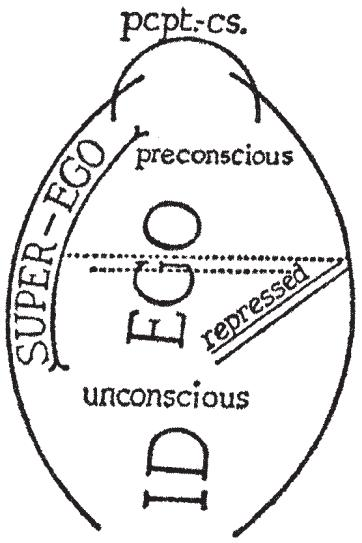
\includegraphics[width=0.72\linewidth]{a9b9ebf53506e9e0115c3e0ac3176d4a0e011804b72ed5e036c409bbfb033975.jpg}
\caption{Freud's structural theory. Freud conceived of three main psychic structures--the ego, the id, and the superego. The ego has a conscious component (perceptual consciousness, or pcpt.-cs.) that receives sensory information and is in direct contact with the outside world, as well as a preconscious component, an aspect of unconscious processing that has ready access to consciousness. The ego's unconscious components act through repression and other defenses to inhibit the instinctual urges of the id, the generator of sexual and aggressive instincts. The ego also responds to the pressures of the superego, the largely unconscious carrier of moral values. The dotted lines indicate the divisions between those processes that are accessible to consciousness and those that are completely unconscious. (From \emph{New Introductory Lectures on Psychoanalysis} [1933]).\\
弗洛伊德的结构理论。弗洛伊德设想了三个主要心理结构：自我、本我和超我。自我有一个意识成分（知觉意识，pcpt.-cs.），它接收感觉信息并与外部世界直接接触；自我还有一个前意识成分，即无意识加工中可较容易进入意识的一个方面。自我的无意识成分通过压抑及其他防御，抑制本我的本能冲动；本我是性本能和攻击本能的发生者。自我也回应超我的压力；超我是道德价值的、在很大程度上无意识的承载者。虚线标示了可进入意识的过程与完全无意识过程之间的分界。（引自《精神分析新引论》[1933]。）}
\end{figure}

\begin{english}
What gave Freud's new model a dramatic turn was the three interacting psychic agencies. Freud did not define the ego, the id, and the superego as either conscious or unconscious, but as differing in cognitive style, goal, and function.
\end{english}
\begin{zhtranslation}
使弗洛伊德新模型产生戏剧性转折的，是这三个相互作用的心理机构。弗洛伊德并没有把自我、本我和超我界定为意识的或无意识的，而是把它们界定为在认知风格、目标和功能上彼此不同。\end{zhtranslation}

\begin{english}
According to Freud's structural theory, the ego (the “I,” or autobiographical self) is the executive agency, and it has both a conscious and an unconscious component. The conscious component is in direct contact with the external world through the sensory apparatus for sight, sound, and touch; it is concerned with perception, reasoning, the planning of action, and the experiencing of pleasure and pain. In their work, Hartmann, Kris, and Lowenstein emphasized that this conflict-free component of the ego operates logically and is guided in its actions by the reality principle. The unconscious component of the ego is concerned with psychological defenses (repression, denial, sublimation), the mechanisms whereby the ego inhibits, channels, and redirects both the sexual and the aggressive instinctual drives of the id, the second psychic agency.
\end{english}
\begin{zhtranslation}
根据弗洛伊德的结构理论，自我（“我”，或自传式自我）是执行机构，并且同时具有意识成分和无意识成分。意识成分通过视觉、听觉和触觉的感觉装置与外部世界直接接触；它涉及知觉、推理、行动计划以及愉悦和痛苦的体验。哈特曼、克里斯和勒文斯坦在其工作中强调，自我这一没有冲突的成分以逻辑方式运行，并在行动中受现实原则引导。自我的无意识成分涉及心理防御（压抑、否认、升华），即自我用来抑制、疏导并重新定向第二个心理机构本我的性本能驱力和攻击本能驱力的机制。\end{zhtranslation}

\begin{english}
The id (the “it”, a term that Freud borrowed from Friedrich Nietzsche, is totally unconscious. It is not governed by logic or by reality but by the hedonistic principle of seeking pleasure and avoiding pain. The id, according to Freud, represents the primitive mind of the infant and is the only mental structure present at birth. The superego, the third governor, is the unconscious moral agency, the embodiment of our aspirations.
\end{english}
\begin{zhtranslation}
本我（“它”）这个术语，是弗洛伊德从弗里德里希·尼采那里借来的；本我是完全无意识的。它不受逻辑或现实支配，而受寻求快乐、避免痛苦的享乐原则支配。按照弗洛伊德的说法，本我代表婴儿的原始心智，是出生时唯一存在的心理结构。第三个统辖者超我，则是无意识的道德机构，是我们理想追求的体现。\end{zhtranslation}

\begin{english}
Although Freud did not intend his diagram to be a neuroanatomical map of mind, it stimulated me to wonder where in the elaborate folds of the human brain these psychic agencies might live, as it had earlier stimulated the curiosity of Kubie and Ostow. As I mentioned, these two psychoanalysts with a keen interest in biology had encouraged me to study with Grundfest.
\end{english}
\begin{zhtranslation}
尽管弗洛伊德并不打算把这幅图当作心智的神经解剖图，它仍激发我去想象，这些心理机构可能居住在人脑复杂褶皱中的什么地方；此前，它也曾激发库比和奥斯托的好奇心。正如我提到过的，这两位对生物学有浓厚兴趣的精神分析学家曾鼓励我跟随格伦德费斯特学习。\end{zhtranslation}

\begin{english}
Grundfest listened patiently as I told him of my rather grandiose ideas. Another biologist might well have dismissed me, wondering what to do with this naive and misguided medical student. But not Grundfest. He explained that my hope of understanding the biological basis of Freud's structural theory of mind was far beyond the grasp of contemporary brain science. Rather, he told me, to understand mind we needed to look at the brain one cell at a time.
\end{english}
\begin{zhtranslation}
我向格伦德费斯特讲述这些相当宏大的想法时，他耐心地听着。换作另一位生物学家，很可能已经把我打发走了，不知道该拿这个天真而误入歧途的医学生怎么办。但格伦德费斯特没有。他解释说，我想理解弗洛伊德心智结构理论的生物学基础，这远远超出了当时脑科学的能力范围。相反，他告诉我，要理解心智，我们需要一次研究大脑中的一个细胞。\end{zhtranslation}

\begin{english}
One cell at a time! I initially found those words demoralizing. How could one address psychoanalytic questions about the unconscious motivation of behavior, or the action of our conscious life, by studying the brain on the level of single nerve cells? But as we talked I suddenly remembered that in 1887, when Freud began his own career, he had sought to solve the hidden riddles of mental life by studying the brain one nerve cell at a time. Freud started out as an anatomist, studying single nerve cells, and had anticipated a key point of what later came to be called the neuron doctrine, the view that nerve cells are the building blocks of the brain. It was only later, after he began treating mentally ill patients in Vienna, that Freud made his monumental discoveries about unconscious mental processes.
\end{english}
\begin{zhtranslation}
一次研究一个细胞！起初我觉得这句话令人沮丧。通过在单个神经细胞层面研究大脑，怎么可能处理精神分析关于行为的无意识动机，或者关于我们意识生活作用的问题呢？但在谈话中，我突然想起，1887年弗洛伊德开始自己的职业生涯时，他正是试图通过一次研究一个神经细胞来解开心理生活的隐秘谜题。弗洛伊德最初是一名解剖学家，研究单个神经细胞；他还预见了后来所谓神经元学说的一个要点，即神经细胞是大脑的构件。只是后来，在维也纳开始治疗精神疾病患者之后，弗洛伊德才作出了关于无意识心理过程的重大并具有里程碑意义的发现。\end{zhtranslation}

\begin{english}
I found it ironic and remarkable that I was now being encouraged to take that journey in reverse, to move from an interest in the top-down structural theory of mind to the bottom-up study of the signaling elements of the nervous system, the intricate inner worlds of nerve cells. Harry Grundfest offered to guide me into this new world.
\end{english}
\begin{zhtranslation}
我觉得既讽刺又非凡的是，现在有人鼓励我反向踏上这段旅程：从对自上而下的心智结构理论的兴趣，转向自下而上地研究神经系统的信号元件，研究神经细胞复杂的内部世界。哈里·格伦德费斯特愿意引导我进入这个新世界。\end{zhtranslation}

\begin{center}
[\dots]
\end{center}

\section*{Chapter 28. Consciousness\\第二十八章 意识}

\begin{english}
Psychoanalysis introduced us to the unconscious in its several forms. Like many scientists now working on the brain, I have long been intrigued by the biggest question about the brain: the nature of consciousness and how various unconscious psychological processes relate to conscious thought. When I first talked with Harry Grundfest about Freud's structural theory of mind--the ego, the id, and the superego--the central focus of my thinking was: How do conscious and unconscious processes differ in their representation in the brain? But only recently has the new science of mind developed the tools for exploring this question experimentally.
\end{english}
\begin{zhtranslation}
精神分析使我们认识了无意识的多种形式。像今天许多研究大脑的科学家一样，我长期以来一直被关于大脑的最大问题所吸引：意识的本性，以及各种无意识心理过程如何与意识思维相关。当我第一次与哈里·格伦德费斯特谈论弗洛伊德的心智结构理论，即自我、本我和超我时，我思考的中心焦点是：意识过程和无意识过程在大脑中的表征有什么不同？但直到最近，新的心智科学才发展出实验探索这个问题的工具。\end{zhtranslation}

\begin{english}
To develop productive insights into consciousness, the new science of mind first had to settle on a working definition of consciousness as a state of perceptual awareness, or selective attention writ large. At its core, consciousness in people is an awareness of self, an awareness of being aware. Consciousness thus refers to our ability not simply to experience pleasure and pain but to attend to and reflect upon those experiences, and to do so in the context of our immediate lives and our life history. Conscious attention allows us to shut out extraneous experiences and focus on the critical event that confronts us, be it pleasure or pain, the blue of the sky, the cool northern light of a Vermeer painting, or the beauty and calm we experience at the seashore.
\end{english}
\begin{zhtranslation}
为了对意识形成有成果的洞见，新的心智科学首先必须确定一个工作性定义：意识是一种知觉觉知状态，或者说是放大了的选择性注意。就其核心而言，人的意识是自我觉知，是对“自己正在觉知”的觉知。因此，意识指的不只是我们体验愉悦和痛苦的能力，还包括我们关注并反思这些体验的能力，并且是在我们当下生活和生命史的语境中这样做的能力。意识注意使我们能够排除无关经验，聚焦于面对我们的关键事件，无论它是愉悦还是痛苦，是天空的蓝色、维米尔画作中清冷的北方光线，还是我们在海边体验到的美与宁静。\end{zhtranslation}

\begin{english}
Understanding consciousness is by far the most challenging task confronting science. The truth of this assertion can best be seen in the career of Francis Crick, perhaps the most creative and influential biologist of the second half of the twentieth century. When Crick first entered biology, after World War II, two great questions were thought to be beyond the capacities of science to answer: What distinguishes the living from the nonliving world? And what is the biological nature of consciousness? Crick turned first to the easier problem, distinguishing animate from inanimate matter, and explored the nature of the gene. By 1953, after just two years of collaboration, he and Jim Watson had helped solve that mystery. As Watson later described in \emph{The Double Helix}, “at lunch Francis winged into the Eagle [Pub] to tell everyone within hearing distance that we had found the secret of life.” In the next two decades, Crick helped crack the genetic code: how DNA makes RNA and RNA makes protein.
\end{english}
\begin{zhtranslation}
理解意识是迄今为止科学所面临的最具挑战性的任务。这一断言的真实性，最好可以从弗朗西斯·克里克的职业生涯中看出；他也许是二十世纪下半叶最富创造力、最有影响力的生物学家。第二次世界大战后，克里克刚进入生物学领域时，人们认为有两个大问题超出了科学能够回答的范围：什么把有生命世界与无生命世界区分开来？意识的生物学本性是什么？克里克首先转向较容易的问题，即区分有生命物质和无生命物质，并探索基因的本性。到1953年，经过仅仅两年的合作，他和吉姆·沃森已经帮助解开了这个谜。正如沃森后来在《双螺旋》中描述的：“午餐时，弗朗西斯飞奔进鹰酒馆，告诉所有听得见的人，我们找到了生命的秘密。”在接下来的二十年里，克里克帮助破解了遗传密码：DNA如何制造RNA，RNA如何制造蛋白质。\end{zhtranslation}

\begin{english}
In 1976, at age sixty, Crick turned to the remaining scientific mystery: the biological nature of consciousness. This he studied for the rest of his life in partnership with Christof Koch, a young computational neuroscientist. Crick brought his characteristic intelligence and optimism to bear on the question; moreover, he made consciousness a focus of the scientific community, which had previously ignored it. But, despite almost thirty years of continuous effort, Crick was able to budge the problem only a modest distance. Indeed, some scientists and philosophers of mind continue to find consciousness so inscrutable that they fear it can never be explained in physical terms. How can a biological system, a biological machine, they ask, feel anything? Even more doubtful, how can it think about itself?
\end{english}
\begin{zhtranslation}
1976年，六十岁的克里克转向剩下的那个科学谜题：意识的生物学本性。此后余生，他与年轻的计算神经科学家克里斯托夫·科赫合作研究这一问题。克里克把他特有的智慧和乐观精神用于这个问题；此外，他使意识成为科学共同体关注的焦点，而此前科学界一直忽视它。但是，尽管持续努力了近三十年，克里克也只把这个问题向前推进了一小段距离。确实，一些科学家和心灵哲学家仍然觉得意识如此不可理解，以至于担心它永远无法用物理术语解释。他们问：一个生物系统、一台生物机器，怎么会有任何感觉？更可疑的是，它怎么会思考自身？
\end{zhtranslation}

\begin{english}
These questions are not new. They were first posed in Western thought during the fifth century B.C. by Hippocrates and by the philosopher Plato, the founder of the Academy in Athens. Hippocrates was the first physician to cast superstition aside, basing his thinking on clinical observations and arguing that all mental processes emanate from the brain. Plato, who rejected observations and experiments, believed that the only reason we can think about ourselves and our mortal body is that we have a soul that is immaterial and immortal. The idea of an immortal soul was subsequently incorporated into Christian thought and elaborated upon by St. Thomas Aquinas in the thirteenth century. Aquinas and later religious thinkers held that the soul--the generator of consciousness--is not only distinct from the body, it is also of divine origin.
\end{english}
\begin{zhtranslation}
这些问题并不新。在西方思想中，它们最早由公元前五世纪的希波克拉底和哲学家柏拉图提出；柏拉图是雅典学园的创立者。希波克拉底是第一个把迷信抛在一边的医生，他把自己的思考建立在临床观察之上，并主张一切心理过程都源自大脑。拒绝观察和实验的柏拉图则认为，我们之所以能够思考自己以及自身会死的身体，唯一原因是我们有一个非物质且不朽的灵魂。不朽灵魂的观念随后被纳入基督教思想，并在十三世纪由圣托马斯·阿奎那加以阐发。阿奎那以及后来的宗教思想家认为，灵魂这个意识的产生者不仅不同于身体，而且具有神圣起源。\end{zhtranslation}

\begin{english}
In the seventeenth century, René Descartes developed the idea that human beings have a dual nature: they have a body, which is made up of material substance, and a mind, which derives from the spiritual nature of the soul. The soul receives signals from the body and can influence its actions but is itself made up of an immaterial substance that is unique to human beings. Descartes' thinking gave rise to the view that actions like eating and walking, as well as sensory perception, appetites, passions, and even simple forms of learning, are all mediated by the brain and can be studied scientifically. Mind, however, is sacred and as such is not a proper subject of science.
\end{english}
\begin{zhtranslation}
十七世纪，勒内·笛卡尔发展出这样一种观念：人具有双重本性。人有身体，由物质实体构成；也有心灵，源自灵魂的精神本性。灵魂接收来自身体的信号，并能影响身体的行动，但灵魂本身由一种人类所独有的非物质实体构成。笛卡尔的思想产生了一种看法，即吃饭、行走等行动，以及感觉知觉、欲望、激情，甚至简单形式的学习，都是由大脑中介的，并且可以被科学研究。然而心灵是神圣的，因此并不是科学的适当对象。\end{zhtranslation}

\begin{english}
It is remarkable to reflect that these seventeenth-century ideas were still current in the 1980s. Karl Popper, the Vienna-born philosopher of science, and John Eccles, the Nobel laureate neurobiologist, espoused dualism all of their lives. They agreed with Aquinas that the soul is immortal and independent of the brain. Gilbert Ryle, the British philosopher of science, referred to the notion of the soul as “the ghost in the machine.”\end{english}
\begin{zhtranslation}
令人惊讶的是，回想起来，这些十七世纪的观念在二十世纪八十年代仍然流行。出生于维也纳的科学哲学家卡尔·波普尔和诺贝尔奖得主、神经生物学家约翰·埃克尔斯，一生都拥护二元论。他们同意阿奎那的观点，认为灵魂不朽并且独立于大脑。英国科学哲学家吉尔伯特·赖尔把灵魂观念称为“机器中的幽灵”。\end{zhtranslation}

\begin{english}
Today, most philosophers of mind agree that what we call consciousness derives from the physical brain, but some disagree with Crick as to whether it can ever be approached scientifically. A few, such as Colin McGinn, believe that consciousness simply cannot be studied, because the architecture of the brain poses limitations on human cognitive capacities. In McGinn's view, the human mind may simply be incapable of solving certain problems. At the other extreme, philosophers such as Daniel Dennett deny that there is any problem at all. Dennett argues, much as neurologist John Hughlings Jackson did a century earlier, that consciousness is not a distinct operation of the brain; rather, it is the combined result of the computational workings of higher-order areas of the brain concerned with later stages of information processing.
\end{english}
\begin{zhtranslation}
今天，多数心灵哲学家都同意，我们所谓的意识来自物理大脑；但在意识是否终究能够以科学方式接近这一点上，有些人不同意克里克。少数人如科林·麦金认为，意识根本无法被研究，因为大脑的结构限制了人类认知能力。在麦金看来，人类心智也许就是不能解决某些问题。另一个极端上，丹尼尔·丹尼特等哲学家则否认这里有任何问题。丹尼特的论证与一个世纪前神经学家约翰·休林斯·杰克逊的论证十分相似：意识并不是大脑的一种独立运作；相反，它是大脑中与信息加工后期阶段有关的高级区域计算活动的综合结果。\end{zhtranslation}

\begin{english}
Finally, philosophers such as John Searle and Thomas Nagel take a middle position, holding that consciousness is a discrete set of biological processes. The processes are accessible to analysis, but we have made little headway in understanding them because they are very complex and represent more than the sum of their parts. Consciousness is therefore much more complicated than any property of the brain that we understand.
\end{english}
\begin{zhtranslation}
最后，约翰·塞尔和托马斯·内格尔等哲学家采取中间立场，认为意识是一组离散的生物过程。这些过程可以被分析，但由于它们非常复杂，并且不只是各部分之和，我们在理解它们方面进展很小。因此，意识比我们所理解的大脑任何性质都复杂得多。\end{zhtranslation}

\begin{english}
Searle and Nagel ascribe two characteristics to the conscious state: unity and subjectivity. The unitary nature of consciousness refers to the fact that our experiences come to us as a unified whole. All of the various sensory modalities are melded into a single, coherent, conscious experience. Thus when I approach a rosebush in the botanical garden at Wave Hill near my house in Riverdale, I sniff the exquisite fragrance of the blossoms at the same time that I see their beautiful red color--and I perceive this rosebush against the background of the Hudson River and the cliffs of the Palisade mountain ridge behind it. My perception is not only whole during the moment I experience it, it is also whole two weeks later, when I engage in mental time travel to recapture the moment. Despite the fact that there are different organs for smell and vision, and that each uses its own individual pathways, they converge in the brain in such a way that my perceptions are unified.
\end{english}
\begin{zhtranslation}
塞尔和内格尔把两个特征归于意识状态：统一性和主观性。意识的统一性是指，我们的经验以统一整体的形式来到我们这里。各种感觉通道都融合为单一、连贯的意识经验。因此，当我走近河谷区我家附近波浪山植物园里的一丛玫瑰时，我一边闻到花朵精致的芳香，一边看到它们美丽的红色；而且我是在以哈德逊河以及其后帕利塞兹山脊的悬崖为背景时知觉到这丛玫瑰的。我的知觉不仅在我体验它的那个瞬间是完整的；两周以后，当我进行心理时间旅行以重新捕捉那个瞬间时，它仍然是完整的。尽管嗅觉和视觉有不同器官，而且各自使用独立通路，它们仍以某种方式在大脑中汇合，使我的知觉成为统一的。\end{zhtranslation}

\begin{english}
The unitary nature of consciousness poses a difficult problem, but perhaps not an insurmountable one. This unitary nature can break down. In a surgical patient whose brain is severed between the two hemispheres, there are two conscious minds, each with its own unified percept.
\end{english}
\begin{zhtranslation}
意识的统一性提出了一个困难问题，但也许不是不可克服的问题。这种统一性可能破裂。在一名两半球之间连接被外科切断的患者那里，会有两个意识心灵，每一个都有自己的统一知觉。\end{zhtranslation}

\begin{english}
Subjectivity, the second characteristic of conscious awareness, poses the more formidable scientific challenge. Each of us experiences a world of private and unique sensations that is much more real to us than the experiences of others. We experience our own ideas, moods, and sensations directly, whereas we can only appreciate another person's experience indirectly, by observing or hearing about it. We therefore can ask, Is your response to the blue you see and the jasmine you smell--the meaning it has for you--identical to my response to the blue I see and the jasmine I smell and the meaning these have for me?
\end{english}
\begin{zhtranslation}
主观性是意识觉知的第二个特征，它提出了更艰巨的科学挑战。我们每个人都体验一个私人而独特的感觉世界；这个世界对我们来说比他人的经验真实得多。我们直接体验自己的观念、情绪和感觉，而只能通过观察或听别人讲述来间接理解另一个人的经验。因此我们可以问：你对你所看见的蓝色和所闻到的茉莉的反应，即它对你的意义，是否与我对我所看见的蓝色和所闻到的茉莉的反应以及它们对我的意义完全相同？
\end{zhtranslation}

\begin{english}
The issue here is not one of perception per se. It is not whether we each see a very similar shade of the same blue. That is relatively easy to establish by recording from single nerve cells in the visual system of different individuals. The brain does reconstruct our perception of an object, but the object perceived--the color blue or middle C on the piano--appears to correspond to the physical properties of the wavelength of the reflected light or the frequency of the emitted sound. Instead, the issue is the significance of that blue and that note for each of us. What we do not understand is how electrical activity in neurons gives rise to the meaning we ascribe to that color or that wavelength of sound. The fact that conscious experience is unique to each person raises the question of whether it is possible to determine objectively any characteristics of consciousness that are common to everyone. If the senses ultimately produce experiences that are completely and personally subjective, we cannot, the argument goes, arrive at a general definition of consciousness based on personal experience.
\end{english}
\begin{zhtranslation}
这里的问题并不是知觉本身的问题。问题不在于我们是否各自看见了同一种蓝色中非常相近的色调。通过记录不同个体视觉系统中单个神经细胞的活动，这一点相对容易确定。大脑确实会重构我们对一个对象的知觉，但被知觉的对象，即蓝色或钢琴上的中央C，似乎对应于反射光波长或发出声音频率的物理性质。相反，问题在于那种蓝色和那个音符对我们每个人的意义。我们不理解的是，神经元中的电活动如何产生我们赋予那种颜色或那一声波波长的意义。意识经验对每个人都是独特的这一事实提出了一个问题：是否可能客观地确定某些对每个人都共同的意识特征？如果感觉最终产生的经验是完全个人化、完全主观的，按照这种论证，我们就不能基于个人经验得出意识的一般定义。\end{zhtranslation}

\begin{english}
Nagel and Searle illustrate the difficulty of explaining the subjective nature of consciousness in physical terms as follows: Assume we succeed in recording the electrical activity of neurons in a region known to be important for consciousness while the person being studied carries out some task that requires conscious attention. For example, suppose we identified the cells that fire when I look at and become aware of a red image of the blossoms on a rosebush at Wave Hill. We have now taken a first step in studying consciousness--namely, we have found what Crick and Koch have called the neural correlate of consciousness for this one percept. For most of us, this would be a great advance because it pinpoints a material concomitant of conscious perception. From there we could go on to carry out experiments to determine whether these correlates also meld into a coherent whole, that is, the background of the Hudson River and the Palisades. But for Nagel and Searle, this is the easy problem of consciousness. The hard problem of consciousness is the second mystery, that of subjective experience.
\end{english}
\begin{zhtranslation}
内格尔和塞尔用如下方式说明以物理术语解释意识主观本性的困难：假定在被研究者执行某项需要意识注意的任务时，我们成功记录了已知对意识重要的某个脑区中神经元的电活动。例如，设想我看见并觉知到波浪山玫瑰丛花朵的红色图像时，我们识别出了放电的细胞。我们现在就迈出了研究意识的第一步，也就是找到了克里克和科赫所说的这一知觉的意识神经相关物。对我们大多数人来说，这会是一项巨大进展，因为它精确指出了意识知觉的一个物质伴随物。由此出发，我们可以继续做实验，确定这些相关物是否也融合为一个连贯整体，即哈德逊河和帕利塞兹的背景。但对内格尔和塞尔来说，这是意识的容易问题。意识的困难问题是第二个谜，即主观经验之谜。\end{zhtranslation}

\begin{english}
How is it that I respond to the red image of a rose with a feeling that is distinctive to me? To use another example, what grounds do we have for believing that when a mother looks at her child, the firing of cells in the region of the cortex concerned with face recognition accounts for the emotions she feels and for her ability to summon the memory of those emotions and that image of her child?
\end{english}
\begin{zhtranslation}
为什么我会以一种对我而言独特的感觉来回应玫瑰的红色图像？再举一个例子，我们有什么根据相信，当一位母亲看着自己的孩子时，皮层中与面孔识别有关区域的细胞放电，就能解释她感受到的情感，以及她唤起这些情感和孩子形象记忆的能力？\end{zhtranslation}

\begin{english}
As yet, we do not know how the firing of specific neurons leads to the subjective component of conscious perception, even in the simplest case. In fact, according to Searle and Nagel, we lack an adequate theory of how an objective phenomenon, such as electrical signals in the brain, can cause a subjective experience, such as pain. And because science as we currently practice it is a reductionist, analytical view of complicated events, while consciousness is irreducibly subjective, such a theory lies beyond our reach for now.
\end{english}
\begin{zhtranslation}
到目前为止，即便在最简单的情形中，我们也不知道特定神经元的放电如何导致意识知觉的主观成分。事实上，按照塞尔和内格尔的说法，我们缺少一种充分理论来解释，一个客观现象，例如大脑中的电信号，如何能够造成一种主观经验，例如疼痛。而且，由于我们当前实践的科学是一种还原论的、分析性的复杂事件观，而意识又不可还原地具有主观性，这样一种理论目前仍超出我们的能力范围。\end{zhtranslation}

\begin{english}
According to Nagel, science cannot take on consciousness without a significant change in methodology, a change that would enable scientists to identify and analyze the elements of subjective experience. Those elements are likely to be basic components of brain function, much as atoms and molecules are basic components of matter, but to exist in a form we cannot yet imagine. The reductions performed routinely in science are not problematic, Nagel holds. Biological science can readily explain how the properties of a particular type of matter arise from the objective properties of the molecules of which it is made. What science lacks are rules for explaining how subjective properties (consciousness) arise from the properties of objects (interconnected nerve cells).
\end{english}
\begin{zhtranslation}
内格尔认为，如果方法论没有重大改变，科学就不能处理意识；这种改变必须使科学家能够识别并分析主观经验的元素。这些元素很可能是大脑功能的基本成分，正如原子和分子是物质的基本成分一样；但它们以一种我们目前还无法想象的形式存在。内格尔认为，科学中常规进行的还原并没有问题。生物科学可以很容易地解释某一特定类型物质的性质如何来自构成它的分子的客观性质。科学所缺少的是一些规则，用来解释主观性质（意识）如何来自对象（相互连接的神经细胞）的性质。\end{zhtranslation}

\begin{english}
Nagel argues that our complete lack of insight into the elements of subjective experience should not prevent us from discovering the neural correlates of consciousness and the rules that relate conscious phenomena to cellular processes in the brain. In fact, it is only by accumulating such information that we will be in a position to think about the reduction of something subjective to something physical and objective. But to arrive at a theory that supports this reduction, we will first have to discover the elements of subjective consciousness. This discovery, says Nagel, will be enormous in its magnitude and its implications, requiring a revolution in biology and most likely a complete transformation of scientific thought.
\end{english}
\begin{zhtranslation}
内格尔主张，尽管我们对主观经验的元素完全缺乏洞见，这不应妨碍我们发现意识的神经相关物，以及把意识现象同大脑中的细胞过程联系起来的规则。事实上，只有通过积累这类信息，我们才会处在能够思考如何把某种主观的东西还原为某种物理而客观的东西的位置上。但是，为了得到一种支持这种还原的理论，我们首先必须发现主观意识的元素。内格尔说，这一发现的规模及其含义将极其巨大，它需要生物学发生一场革命，并且很可能需要科学思想的彻底转变。\end{zhtranslation}

\begin{english}
The aim of most neural scientists working on consciousness is much more modest than this grand perspective would imply. They are not deliberately working toward or anticipating a revolution in scientific thought. Although they must struggle with the difficulties of defining conscious phenomena experimentally, they do not see those difficulties as precluding all experimental study under existing paradigms. Neural scientists believe, and Searle for one agrees with them, that they have been able to make considerable progress in understanding the neurobiology of perception and memory without having to account for individual experience. For example, cognitive neural scientists have made advances in understanding the neural basis of the perception of the color blue without addressing the question of how each of us responds to the same blue.
\end{english}
\begin{zhtranslation}
大多数研究意识的神经科学家的目标，比这种宏大图景所暗示的要谦逊得多。他们并没有有意朝着科学思想革命工作，也没有预期这样的革命。虽然他们必须努力应对以实验方式界定意识现象的困难，但他们并不认为这些困难会排除在现有范式下进行一切实验研究。神经科学家相信，塞尔本人也同意他们，他们已经能够在不解释个人经验的情况下，在理解知觉和记忆的神经生物学方面取得相当进展。例如，认知神经科学家在理解蓝色知觉的神经基础方面取得了进展，而没有处理我们每个人如何回应同一种蓝色的问题。\end{zhtranslation}

\begin{english}
What we do not understand is the hard problem of consciousness--the mystery of how neural activity gives rise to subjective experience. Crick and Koch have argued that once we solve the easy problem of consciousness, the unity of consciousness, we will be able to manipulate those neural systems experimentally to solve the hard problem.
\end{english}
\begin{zhtranslation}
我们所不理解的，是意识的困难问题，即神经活动如何产生主观经验之谜。克里克和科赫认为，一旦我们解决了意识的容易问题，也就是意识的统一性，我们就能够通过实验操纵那些神经系统，从而解决困难问题。\end{zhtranslation}

\begin{english}
The unity of consciousness is a variant of the binding problem first identified in the study of visual perception. An intimate part of my experiencing the subjective pleasure of the moment at Wave Hill is how the look and the smell of roses in the gardens are bound together and unified with my view of the Hudson, the Palisades, and all the other component images of my perception. Each of these components of my subjective experience is mediated by different brain regions within my visual, olfactory, and emotional systems. The unity of my conscious experience implies that the binding process must somehow connect and integrate all of these separate areas in the brain.
\end{english}
\begin{zhtranslation}
意识的统一性是最初在视觉知觉研究中被识别出的绑定问题的一种变体。我在波浪山那个时刻体验到主观愉悦，其中一个亲密组成部分，就是花园中玫瑰的外观和气味如何与我对哈德逊河、帕利塞兹以及我知觉中所有其他组成图像的观看绑定在一起并统一起来。我的主观经验中每一个组成部分，都是由视觉、嗅觉和情感系统中的不同脑区中介的。我的意识经验的统一性意味着，绑定过程必须以某种方式把大脑中所有这些分离区域连接并整合起来。\end{zhtranslation}

\begin{english}
As a first step toward solving the easy problem of consciousness, we need to ask whether the unity of consciousness--a unity thought to be achieved by neural systems that mediate selective attention--is localized in one or just a few sites, which would enable us to manipulate them biologically. The answer to this question is by no means clear. Gerald Edelman, a leading theoretician on the brain and consciousness, has argued effectively that the neural machinery for the unity of consciousness is likely to be widely distributed throughout the cortex and thalamus. As a result, Edelman asserts, it is unlikely that we will be able to find consciousness through a simple set of neural correlates. Crick and Koch, on the other hand, believe that the unity of consciousness will have direct neural correlates because they most likely involve a specific set of neurons with specific molecular or neuroanatomical signatures. The neural correlates, they argue, probably require only a small set of neurons acting as a searchlight: the spotlight of attention. The initial task, they argue, is to locate within the brain that small set of neurons whose activity correlates best with the unity of conscious experience and then to determine the neural circuits to which they belong.
\end{english}
\begin{zhtranslation}
作为解决意识容易问题的第一步，我们需要问：意识的统一性，即被认为由中介选择性注意的神经系统实现的统一性，是否定位在一个或少数几个部位，从而使我们能够以生物学方式操纵它们？这个问题的答案远不清楚。杰拉尔德·埃德尔曼是大脑和意识领域的重要理论家，他有力地论证说，意识统一性的神经机制很可能广泛分布于整个皮层和丘脑。因此，埃德尔曼断言，我们不大可能通过一组简单的神经相关物找到意识。另一方面，克里克和科赫相信，意识的统一性会有直接的神经相关物，因为它们很可能涉及一组具有特定分子或神经解剖标志的神经元。他们认为，这些神经相关物也许只需要一小组像探照灯一样起作用的神经元：注意的聚光灯。他们认为，最初的任务是在大脑中定位那一小组神经元，其活动与意识经验的统一性最为相关，然后确定它们所属的神经回路。\end{zhtranslation}

\begin{english}
How are we to find this small population of nerve cells that could mediate the unity of consciousness? What criteria must they meet? In Crick and Koch's last paper (which Crick was still correcting on his way to the hospital a few hours before he died, on July 28, 2004), they focused on the claustrum, a sheet of brain tissue that is located below the cerebral cortex, as the site that mediates unity of experience. Little is known about the claustrum except that it connects to and exchanges information with almost all of the sensory and motor regions of the cortex as well as the amygdala, which plays an important role in emotion. Crick and Koch compare the claustrum to the conductor of an orchestra. Indeed, the neuroanatomical connections of the claustrum meet the requirements of a conductor; it can bind together and coordinate the various brain regions necessary for the unity of conscious awareness.
\end{english}
\begin{zhtranslation}
我们怎样找到这一小群可能中介意识统一性的神经细胞？它们必须满足什么标准？在克里克和科赫的最后一篇论文中（克里克在2004年7月28日去世前几小时、去医院的路上仍在修改这篇论文），他们把注意力集中在屏状核上。屏状核是位于大脑皮层下方的一片脑组织，被他们视为中介经验统一性的部位。关于屏状核，人们所知甚少；只知道它与皮层几乎所有感觉和运动区域以及杏仁核相连接并交换信息，而杏仁核在情绪中发挥重要作用。克里克和科赫把屏状核比作乐队指挥。确实，屏状核的神经解剖连接符合指挥的要求；它能够把意识觉知统一性所需的各个脑区绑定并协调起来。\end{zhtranslation}

\begin{english}
The idea that obsessed Crick at the end of his life--that the claustrum is the spotlight of attention, the site that binds the various components of any percept together--is the last in a series of important ideas he advanced. Crick's enormous contributions to biology (the double helical structure of DNA, the nature of the genetic code, the discovery of messenger RNA, the mechanisms of translating messenger RNA into the amino acid sequence of a protein, and the legitimizing of the biology of consciousness) put him in a class with Copernicus, Newton, Darwin, and Einstein. Yet his intense, lifelong focus on science, on the life of mind, is something he shares with many in the scientific community, and that obsession is symbolic of science at its best. The cognitive psychologist Vilayanur Ramachandran, a friend and colleague of Crick's, described Crick's focus on the claustrum during his last weeks:
\end{english}
\begin{zhtranslation}
克里克生命末期一直着迷的那个想法，即屏状核是注意的聚光灯，是把任何知觉的各个组成部分绑定在一起的部位，是他提出的一系列重要思想中的最后一个。克里克对生物学的巨大贡献，包括DNA双螺旋结构、遗传密码的本性、信使RNA的发现、把信使RNA翻译成蛋白质氨基酸序列的机制，以及使意识生物学获得合法地位，使他跻身哥白尼、牛顿、达尔文和爱因斯坦之列。然而，他对科学、对心智生命的强烈而终生的专注，是他与科学共同体中许多人共享的东西；这种执着象征着科学最好的样子。克里克的朋友和同事、认知心理学家维拉亚努尔·拉马钱德兰，描述了克里克生命最后几周对屏状核的关注。\end{zhtranslation}

\begin{english}
Three weeks prior to his death I visited him in his home in La Jolla. He was eighty-eight, had terminal cancer, was in pain, and was on chemotherapy; yet he had obviously been working away nonstop on his latest project. His very large desk--occupying half the room--was covered by articles, correspondence, envelopes, recent issues of \emph{Nature}, a laptop (despite his dislike of computers), and recent books on neuroanatomy. During the whole two hours that I was there, there was no mention of his illness--only a flight of ideas on the neural basis of consciousness. He was especially interested in a tiny structure called the claustrum which, he felt, had been largely ignored by mainstream pundits. As I was leaving he said: “Rama, I think the secret of consciousness lies in the claustrum--don't you? Why else would this tiny structure be connected to so many areas in the brain?” And gave me a sly, conspiratorial wink. It was the last time I saw him.
\end{english}
\begin{zhtranslation}
他去世前三周，我到拉霍亚的家中拜访他。他八十八岁，患有晚期癌症，忍受疼痛，并正在接受化疗；然而很明显，他一直不停地投入到最新项目中。他那张很大的书桌占了半个房间，上面堆满论文、信件、信封、近期的《自然》杂志、一台笔记本电脑（尽管他不喜欢电脑），以及新近出版的神经解剖学书籍。我在那里待了整整两个小时，期间没有提到他的病情，只有关于意识神经基础的思想飞翔。他特别感兴趣的是一个叫屏状核的微小结构，他觉得主流权威大多忽视了它。我离开时，他说：“拉玛，我认为意识的秘密就在屏状核里，你不这么想吗？否则为什么这个微小结构会连接到大脑这么多区域？”然后给了我一个狡黠、像同谋般的眨眼。那是我最后一次见到他。\end{zhtranslation}

\begin{english}
Since so little is known about the claustrum, Crick continued, he wanted to start an institute to focus on its function. In particular, he wanted to determine whether the claustrum is switched on when unconscious, subliminal perception of a given stimulus by a person's sensory organs turns into a conscious percept.
\end{english}
\begin{zhtranslation}
克里克接着说，由于关于屏状核所知太少，他想创办一个研究所，专门关注它的功能。尤其是，他想确定，当一个人的感觉器官对某个给定刺激的无意识、潜意识知觉转变为一个意识知觉时，屏状核是否被开启。\end{zhtranslation}

\begin{english}
One example of such switching that intrigued Crick and Koch is binocular rivalry. Here, two different images--say, vertical stripes and horizontal stripes--are presented to a person simultaneously in such a way that each eye sees only one set of stripes. The person may combine the two images and report seeing a plaid, but more commonly the person will see first one image, then the next, with horizontal and vertical stripes alternating back and forth spontaneously.
\end{english}
\begin{zhtranslation}
令克里克和科赫感兴趣的这种切换的一个例子是双眼竞争。在这种情形中，两种不同图像，例如竖条纹和横条纹，同时呈现给一个人，但呈现方式使每只眼睛只看见一组条纹。这个人可能把两幅图像合并起来，并报告说看见了格子图案；但更常见的是，他会先看见一幅图像，随后看见另一幅图像，横条纹和竖条纹自发地来回交替。\end{zhtranslation}

\begin{english}
Using MRI, Eric Lumer and his colleagues at University College, London have identified the frontal and parietal areas of the cortex as the regions of the brain that become active when a person's conscious attention switches from one image to another. These two regions have a special role in focusing conscious attention on objects in space. In turn, the prefrontal and posterior parietal regions of the cortex seem to relay the decision regarding which image is to be enhanced to the visual system, which then brings the image into consciousness. Indeed, people with damage to the prefrontal cortex have difficulty switching from one image to the other in situations of binocular rivalry. Crick and Koch might argue that the frontal and parietal areas of the cortex are recruited by the claustrum, which switches attention from one eye to the other and unifies the image presented to conscious awareness by each eye.
\end{english}
\begin{zhtranslation}
伦敦大学学院的埃里克·卢默及其同事利用MRI发现，当一个人的意识注意从一幅图像切换到另一幅图像时，皮层的额叶和顶叶区域会被激活。这两个区域在把意识注意聚焦于空间中的对象方面具有特殊作用。随后，皮层前额叶和后顶叶区域似乎把“哪一幅图像应当被增强”的决定传递给视觉系统，视觉系统再把该图像带入意识。事实上，前额叶皮层受损的人在双眼竞争情形中难以从一幅图像切换到另一幅图像。克里克和科赫也许会说，皮层额叶和顶叶区域是由屏状核招募的；屏状核把注意从一只眼切换到另一只眼，并统一每只眼呈现给意识觉知的图像。\end{zhtranslation}

\begin{english}
As these arguments make clear, consciousness remains an enormous problem. But through the efforts of Edelman on the one hand, and Crick and Koch on the other, we now have two specific and testable theories worthy of exploration.
\end{english}
\begin{zhtranslation}
正如这些论证所表明的，意识仍然是一个巨大的问题。但是，一方面通过埃德尔曼的努力，另一方面通过克里克和科赫的努力，我们现在拥有了两个具体且可检验、值得探索的理论。\end{zhtranslation}

\begin{english}
As someone interested in psychoanalysis, I wanted to take the Crick-Koch paradigm of comparing unconscious and conscious perception of the same stimulus to the next step: determining how visual perception becomes endowed with emotion. Unlike simple visual perception, emotionally charged visual perception is likely to differ between individuals. Therefore, a further question is, How and where are unconscious emotional perceptions processed?
\end{english}
\begin{zhtranslation}
作为一个对精神分析感兴趣的人，我想把克里克-科赫比较同一刺激的无意识知觉和意识知觉的范式推进到下一步：确定视觉知觉如何获得情绪色彩。不同于简单视觉知觉，带有情绪负荷的视觉知觉很可能因人而异。因此，进一步的问题是：无意识的情绪知觉在何处、以何种方式被加工？
\end{zhtranslation}

\begin{english}
Amit Etkin, a bold and creative M.D.-Ph.D. student, and I undertook a study in collaboration with Joy Hirsch, a brain imager at Columbia, in which we induced conscious and unconscious perceptions of emotional stimuli. Our approach paralleled in the emotional sphere that of Crick and Koch in the cognitive sphere. We explored how normal people respond consciously and unconsciously to pictures of people with a clearly neutral expression or an expression of fear on their faces. The pictures were provided by Peter Ekman at the University of California, San Francisco.
\end{english}
\begin{zhtranslation}
阿米特·埃特金是一名大胆而富有创造力的医学博士/哲学博士项目学生，我和他与哥伦比亚大学脑成像专家乔伊·赫希合作开展了一项研究，在其中诱发对情绪刺激的意识知觉和无意识知觉。我们在情绪领域采取的方法，平行于克里克和科赫在认知领域的方法。我们探索正常人如何以意识和无意识方式回应一些人的照片；这些人脸上带有明确的中性表情或恐惧表情。照片由加利福尼亚大学旧金山分校的保罗·艾克曼提供。\end{zhtranslation}

\begin{english}
Ekman, who has cataloged more than 100,000 human expressions, was able to show, as did Charles Darwin before him, that irrespective of sex or culture, conscious perceptions of seven facial expressions--happiness, fear, disgust, contempt, anger, surprise, and sadness--have virtually the same meaning to everyone (figure 28-1). We therefore argued that fearful faces should elicit a similar response from the healthy young medical and graduate student volunteers in our study, regardless of whether they perceived the stimulus consciously or unconsciously. We produced a conscious perception of fear by presenting the fearful faces for a long period, so people had time to reflect on them. We produced unconscious perception of fear by presenting the same faces so rapidly that the volunteers were unable to report which type of expression they had seen. Indeed, they were not even sure they had seen a face!
\end{english}
\begin{zhtranslation}
艾克曼已经编目了十万多种人类表情；他能够像此前的查尔斯·达尔文一样表明，不论性别或文化，七种面部表情，即快乐、恐惧、厌恶、轻蔑、愤怒、惊讶和悲伤，在意识知觉中对每个人实际上具有相同意义（图28-1）。因此我们认为，恐惧面孔应当在我们研究中的健康年轻医学生和研究生志愿者身上引发类似反应，无论他们是以意识方式还是无意识方式知觉到刺激。我们通过长时间呈现恐惧面孔来产生对恐惧的意识知觉，使人们有时间对它们进行反思。我们通过极快地呈现同样的面孔来产生对恐惧的无意识知觉，快到志愿者无法报告自己看见了哪一种表情。事实上，他们甚至不确定自己看见了一张脸。\end{zhtranslation}

\begin{figure}[htbp]
\centering
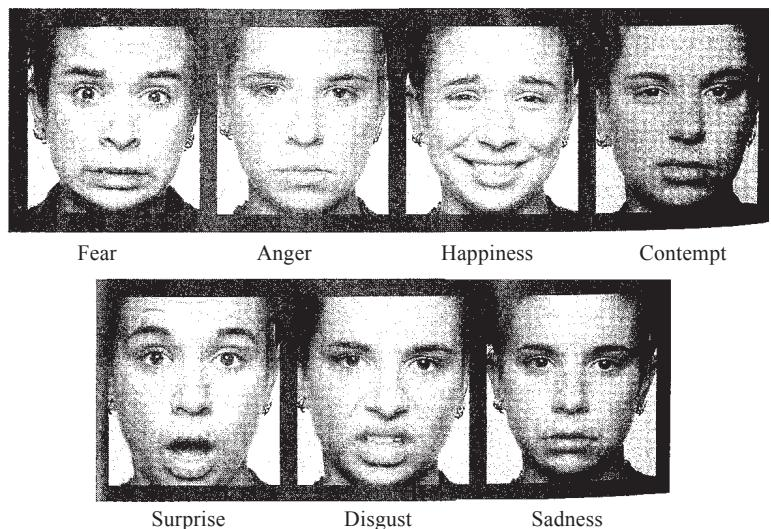
\includegraphics[width=0.8\linewidth]{983d9daa0542de65f607fe473e33e0b93324598b87b96544aac66a41c60daf77.jpg}
\caption{Ekman's seven universal facial expressions. (Courtesy of Paul Ekman.)\\艾克曼的七种普遍面部表情。（保罗·艾克曼惠允。）}
\end{figure}

\begin{english}
Since even normal people differ in their sensitivity to a threat, we gave all of the volunteers a questionnaire designed to measure background anxiety. In contrast to the momentary anxiety most people feel in a new situation, background anxiety reflects an enduring baseline trait.
\end{english}
\begin{zhtranslation}
由于即使正常人对威胁的敏感性也有差异，我们给所有志愿者发放了一份问卷，用来测量背景焦虑。与多数人在新情境中感到的瞬时焦虑不同，背景焦虑反映的是一种持久的基线特质。\end{zhtranslation}

\begin{english}
Not surprisingly, when we showed the volunteers pictures of faces with fearful expressions, we found prominent activity in the amygdala, the structure deep in the brain that mediates fear. What was surprising was that conscious and unconscious stimuli affected different regions of the amygdala, and they did so to differing degrees in different people, depending on their baseline anxiety.
\end{english}
\begin{zhtranslation}
不出所料，当我们向志愿者展示带有恐惧表情的面孔图片时，我们发现杏仁核有显著活动；杏仁核是位于大脑深部、中介恐惧的结构。令人惊讶的是，意识刺激和无意识刺激影响了杏仁核的不同区域，而且它们在不同人身上的影响程度也不同，这取决于他们的基线焦虑。\end{zhtranslation}

\begin{english}
Unconscious perception of fearful faces activated the basolateral nucleus. In people, as in mice, this area of the amygdala receives most of the incoming sensory information and is the primary means by which the amygdala communicates with the cortex. Activation of the basolateral nucleus by unconscious perception of fearful faces occurred in direct proportion to a person's background anxiety: the higher the measure of background anxiety, the greater the person's response. People with low background anxiety had no response at all. Conscious perception of fearful faces, in contrast, activated the dorsal region of the amygdala, which contains the central nucleus, and it did so regardless of a person's background anxiety. The central nucleus of the amygdala sends information to regions of the brain that are part of the autonomic nervous system--concerned with arousal and defensive responses. In sum, unconsciously perceived threats disproportionately affect people with high background anxiety, whereas consciously perceived threats activate the fight-or-flight response in all volunteers.
\end{english}
\begin{zhtranslation}
对恐惧面孔的无意识知觉激活了基底外侧核。在人类和小鼠中一样，杏仁核的这一区域接收大多数传入感觉信息，也是杏仁核与皮层交流的主要通道。由恐惧面孔无意识知觉引起的基底外侧核激活，与一个人的背景焦虑成正比：背景焦虑测量值越高，反应越强。背景焦虑低的人完全没有反应。相反，对恐惧面孔的意识知觉激活了杏仁核背侧区域，其中包含中央核；而且这种激活不受一个人背景焦虑的影响。杏仁核中央核把信息发送到大脑中属于自主神经系统的区域，这些区域与唤醒和防御反应有关。总之，无意识知觉到的威胁不成比例地影响背景焦虑高的人，而意识知觉到的威胁则在所有志愿者中激活战斗或逃跑反应。\end{zhtranslation}

\begin{english}
We also found that unconscious and conscious perception of fearful faces activates different neural networks outside the amygdala. Here again, the networks activated by unconsciously perceived threats were recruited only by the anxious volunteers. Surprisingly, even unconscious perception recruits participation of regions within the cerebral cortex.
\end{english}
\begin{zhtranslation}
我们还发现，对恐惧面孔的无意识知觉和意识知觉，会激活杏仁核之外的不同神经网络。在这里同样，由无意识知觉到的威胁激活的网络，只在焦虑志愿者中被招募。令人惊讶的是，即便无意识知觉也会招募大脑皮层内区域的参与。\end{zhtranslation}

\begin{english}
Thus viewing frightening stimuli activates two different brain systems, one that involves conscious, presumably top-down attention and one that involves unconscious, bottom-up attention, or vigilance, much as a signal of salience does in explicit and implicit memory in \emph{Aplysia} and in the mouse.
\end{english}
\begin{zhtranslation}
因此，观看令人恐惧的刺激会激活两个不同的大脑系统：一个涉及意识的、推测为自上而下的注意；另一个涉及无意识的、自下而上的注意或警觉。这很像显著性信号在海兔和小鼠的外显记忆与内隐记忆中所起的作用。\end{zhtranslation}

\begin{english}
These are fascinating results. First, they show that in the realm of emotion, as in the realm of perception, a stimulus can be perceived both unconsciously and consciously. They also support Crick and Koch's idea that in perception, distinct areas of the brain are correlated with conscious and unconscious awareness of a stimulus. Second, these studies confirm biologically the importance of the psychoanalytic idea of unconscious emotion. They suggest that the effects of anxiety are exerted most dramatically in the brain when the stimulus is left to the imagination rather than when it is perceived consciously. Once the image of a frightened face is confronted consciously, even anxious people can accurately appraise whether it truly poses a threat.
\end{english}
\begin{zhtranslation}
这些结果十分迷人。第一，它们表明，在情绪领域和知觉领域一样，一个刺激既可以被无意识地知觉，也可以被意识地知觉。它们还支持克里克和科赫的想法，即在知觉中，大脑不同区域与对刺激的意识觉知和无意识觉知相关。第二，这些研究从生物学上确认了精神分析中无意识情绪观念的重要性。它们提示，当刺激留给想象而不是被意识地知觉时，焦虑的影响在大脑中表现得最为剧烈。一旦恐惧面孔的图像被意识地面对，即使焦虑的人也能准确评估它是否真正构成威胁。\end{zhtranslation}

\begin{english}
A century after Freud suggested that psychopathology arises from conflict occurring on an unconscious level and that it can be regulated if the source of the conflict is confronted consciously, our imaging studies suggest ways in which such conflicting processes may be mediated in the brain. Moreover, the discovery of a correlation between volunteers' background anxiety and their unconscious neural processes validates biologically the Freudian idea that unconscious mental processes are part of the brain's system of information processing. While Freud's ideas have existed for more than one hundred years, no previous brain-imaging study had tried to account for how differences in people's behavior and interpretations of the world arise from differences in how they unconsciously process emotion. The finding that unconscious perception of fear lights up the basolateral nucleus of the amygdala in direct proportion to a person's baseline anxiety provides a biological marker for diagnosing an anxiety state and for evaluating the efficacy of various drugs and forms of psychotherapy.
\end{english}
\begin{zhtranslation}
在弗洛伊德提出精神病理源自无意识层面的冲突、而如果冲突源头被意识地面对就可以得到调节一个世纪之后，我们的成像研究提示了这类冲突过程可能如何在大脑中被中介。此外，志愿者背景焦虑与其无意识神经过程之间相关性的发现，从生物学上验证了弗洛伊德的思想：无意识心理过程是大脑信息加工系统的一部分。尽管弗洛伊德的思想已经存在一百多年，以前没有脑成像研究试图解释，人们行为和世界解释方式的差异如何来自他们无意识加工情绪方式的差异。无意识知觉恐惧会按一个人基线焦虑的比例点亮杏仁核基底外侧核，这一发现为诊断焦虑状态以及评价各种药物和心理治疗形式的疗效提供了一个生物学标志物。\end{zhtranslation}

\begin{english}
In discerning a correlation between the activity of a neural circuit and the unconscious and conscious perception of a threat, we are beginning to delineate the neural correlate of an emotion--fear. That description might well lead us to a scientific explanation of consciously perceived fear. It might give us an approximation of how neural events give rise to a mental event that enters our awareness. Thus, a half century after I left psychoanalysis for the biology of mind, the new biology of mind is getting ready to tackle some of the issues central to psychoanalysis and consciousness.
\end{english}
\begin{zhtranslation}
通过辨识一个神经回路的活动与对威胁的无意识知觉和意识知觉之间的相关性，我们正开始勾勒一种情绪，即恐惧的神经相关物。这种描述很可能引导我们对意识知觉到的恐惧作出科学解释。它也许能使我们近似地了解，神经事件如何产生一个进入我们觉知的心理事件。因此，在我离开精神分析、转向心智生物学半个世纪之后，新的心智生物学正准备处理某些对精神分析和意识而言居于中心地位的问题。\end{zhtranslation}

\begin{english}
One such issue is the nature of free will. Given Freud's discovery of psychic determinism--the fact that much of our cognitive and affective life is unconscious--what is left for personal choice, for freedom of action?
\end{english}
\begin{zhtranslation}
其中一个问题是自由意志的本性。鉴于弗洛伊德发现了心理决定论，即我们的认知生活和情感生活很大一部分是无意识的，那么个人选择、行动自由还剩下什么？
\end{zhtranslation}

\begin{english}
A critical set of experiments on this question was carried out in 1983 by Benjamin Libet at the University of California, San Francisco. Libet used as his starting point a discovery made by the German neuroscientist Hans Kornhuber. In his study, Kornhuber asked volunteers to move their right index finger. He then measured this voluntary movement with a strain gauge while at the same time recording the electrical activity of the brain by means of an electrode on the skull. After hundreds of trials, Kornhuber found that, invariably, each movement was preceded by a little blip in the electrical record from the brain, a spark of free will! He called this potential in the brain the “readiness potential” and found that it occurred one second before the voluntary movement.
\end{english}
\begin{zhtranslation}
关于这个问题的一组关键实验，是本杰明·利贝特于1983年在加利福尼亚大学旧金山分校完成的。利贝特以德国神经科学家汉斯·科恩胡伯的一项发现为出发点。在科恩胡伯的研究中，他要求志愿者移动右手食指。随后，他用应变计测量这种自主运动，同时通过头骨上的电极记录大脑电活动。经过数百次试验，科恩胡伯发现，每一次运动之前，大脑电记录中总会有一个小小的波动，一点自由意志的火花！他把大脑中的这种电位称为“准备电位”，并发现它发生在自主运动前一秒。\end{zhtranslation}

\begin{english}
Libet followed up on Kornhuber's finding with an experiment in which he asked volunteers to lift a finger whenever they felt the urge to do so. He placed an electrode on a volunteer's skull and confirmed a readiness potential about one second before the person lifted his or her finger. He then compared the time it took for the person to will the movement with the time of the readiness potential. Amazingly, Libet found that the readiness potential appeared not after, but 200 milliseconds before a person felt the urge to move his or her finger! Thus by merely observing the electrical activity of the brain, Libet could predict what a person would do before the person was actually aware of having decided to do it.
\end{english}
\begin{zhtranslation}
利贝特沿着科恩胡伯的发现继续研究，设计了一个实验：他要求志愿者在任何感到有冲动时抬起一根手指。他在志愿者头骨上放置电极，确认在这个人抬起手指前约一秒出现准备电位。随后，他把这个人产生行动意愿所需的时间与准备电位出现的时间进行比较。令人惊讶的是，利贝特发现，准备电位不是出现在一个人感到有冲动移动手指之后，而是出现在此前200毫秒！因此，仅仅通过观察大脑电活动，利贝特就能在一个人实际意识到自己已经决定要做某事之前，预测这个人会做什么。\end{zhtranslation}

\begin{english}
This finding has caused philosophers of mind to ask: If the choice is determined in the brain before we decide to act, where is free will? Is our sense of willing our movements only an illusion, a rationalization after the fact for what has happened? Or is the choice made freely, but not consciously? If so, choice in action, as in perception, may reflect the importance of unconscious inference. Libet proposes that the process of initiating a voluntary action occurs in an unconscious part of the brain, but that just before the action is initiated, consciousness is recruited to approve or veto the action. In the 200 milliseconds before a finger is lifted, consciousness determines whether it moves or not.
\end{english}
\begin{zhtranslation}
这一发现促使心灵哲学家发问：如果选择在我们决定行动之前就已经由大脑决定，那么自由意志在哪里？我们对自己意愿运动的感觉，是否只是一个幻觉，是对已经发生之事的事后合理化？或者，选择是自由作出的，但不是意识地作出的？如果是这样，行动中的选择就可能像知觉一样，反映无意识推理的重要性。利贝特提出，自主行动的启动过程发生在大脑的一个无意识部分，但在行动真正开始前，意识被招募来批准或否决该行动。在手指被抬起前200毫秒内，意识决定它是否移动。\end{zhtranslation}

\begin{english}
Whatever the reasons for the delay between decision and awareness, Libet's findings also raise the moral question: How can one be held responsible for decisions that are made without conscious awareness? The psychologists Richard Gregory and Vilayanur Ramachandran have drawn strict limits on that argument. They point out that “our conscious mind may not have free will, but it does have free won't.” Michael Gazzaniga, one of the pioneers in the development of cognitive neuroscience and a member of the American Council of Bioethics, has added, “Brains are automatic, but people are free.” One cannot infer the sum total of neural activity simply by looking at a few neural circuits in the brain.
\end{english}
\begin{zhtranslation}
无论决定与觉知之间延迟的原因是什么，利贝特的发现也提出了一个道德问题：一个人怎样能为没有意识觉知时作出的决定负责？心理学家理查德·格雷戈里和维拉亚努尔·拉马钱德兰为这种论证划定了严格界限。他们指出：“我们的意识心灵也许没有自由意志，但它确实有自由否决。”认知神经科学发展的先驱之一、美国生物伦理委员会成员迈克尔·加扎尼加又补充说：“大脑是自动的，但人是自由的。”不能仅仅通过观察大脑中的少数神经回路，就推断神经活动的总和。\end{zhtranslation}

\end{document}

